\section{Results}

In this section we present the numerical results obtained for the Poisson problem model using both linear (CST) and quadratic (LST) triangular elements. We generate a sequence of uniform and geometrically graded meshes (controlled by the progression parameter $r = [1.0, 1.05, 1.1]$ and the parameter $\alpha = 3$) and assemble the corresponding finite element systems by exact integration of the element stiffness matrices. After enforcing homogeneous Dirichlet conditions, we solve each sparse linear system to obtain the discrete solution \(u_h\). We then compute the energy norm error \(\|u - u_h\|_{H^1(\Omega)}\) against the known analytic solution and plot its decay versus the mesh size \(h\) on a log–log scale. By fitting a straight line to these data, we extract the observed convergence rates and compare them to the theoretical predictions of \(\mathcal{O}(h^1)\) for CST and \(\mathcal{O}(h^2)\) for LST. Tables and figures below summarize these findings for both uniform and graded discretizations.  

\subsection{CST annalysis}

\begin{figure}[H]
\centering
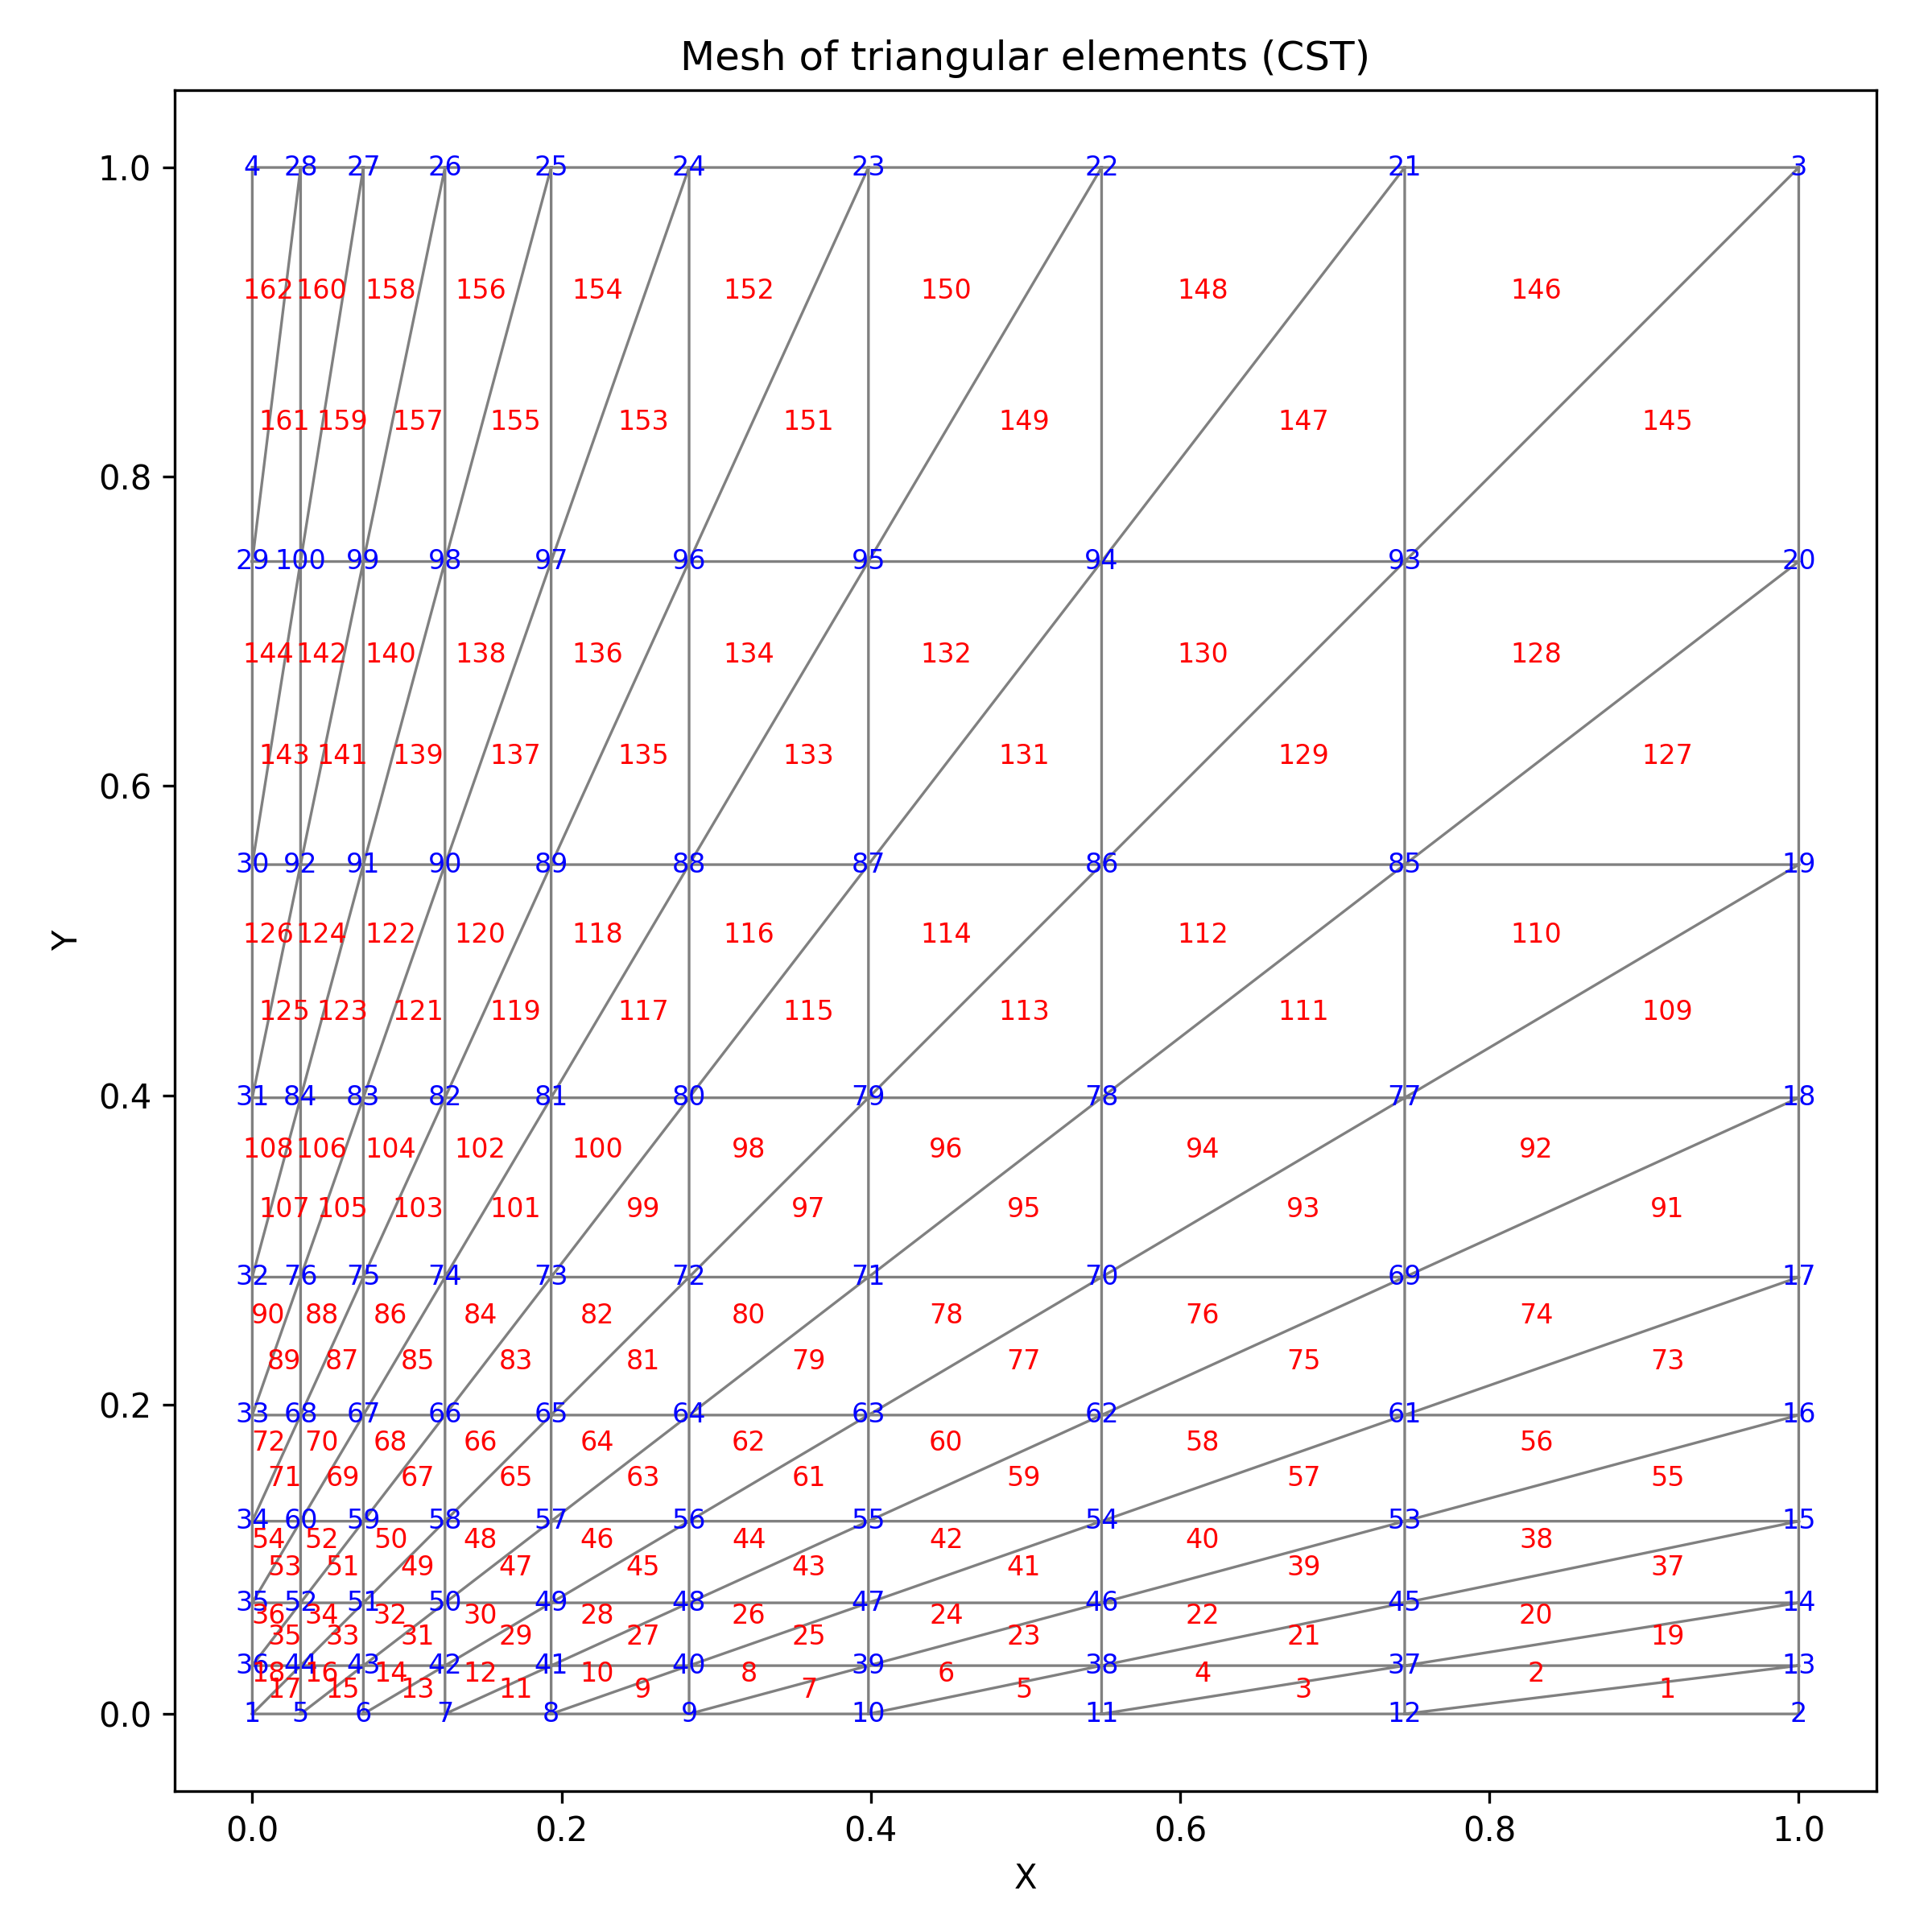
\includegraphics[width=0.4\textwidth]{GRAFICOS/CST/CST_mesh_plot.png}
\caption{CST Mesh}
\label{fig:cst_results}
\end{figure}

\begin{figure}[H]
  \centering
  \begin{subfigure}[b]{0.48\textwidth}
    \centering
    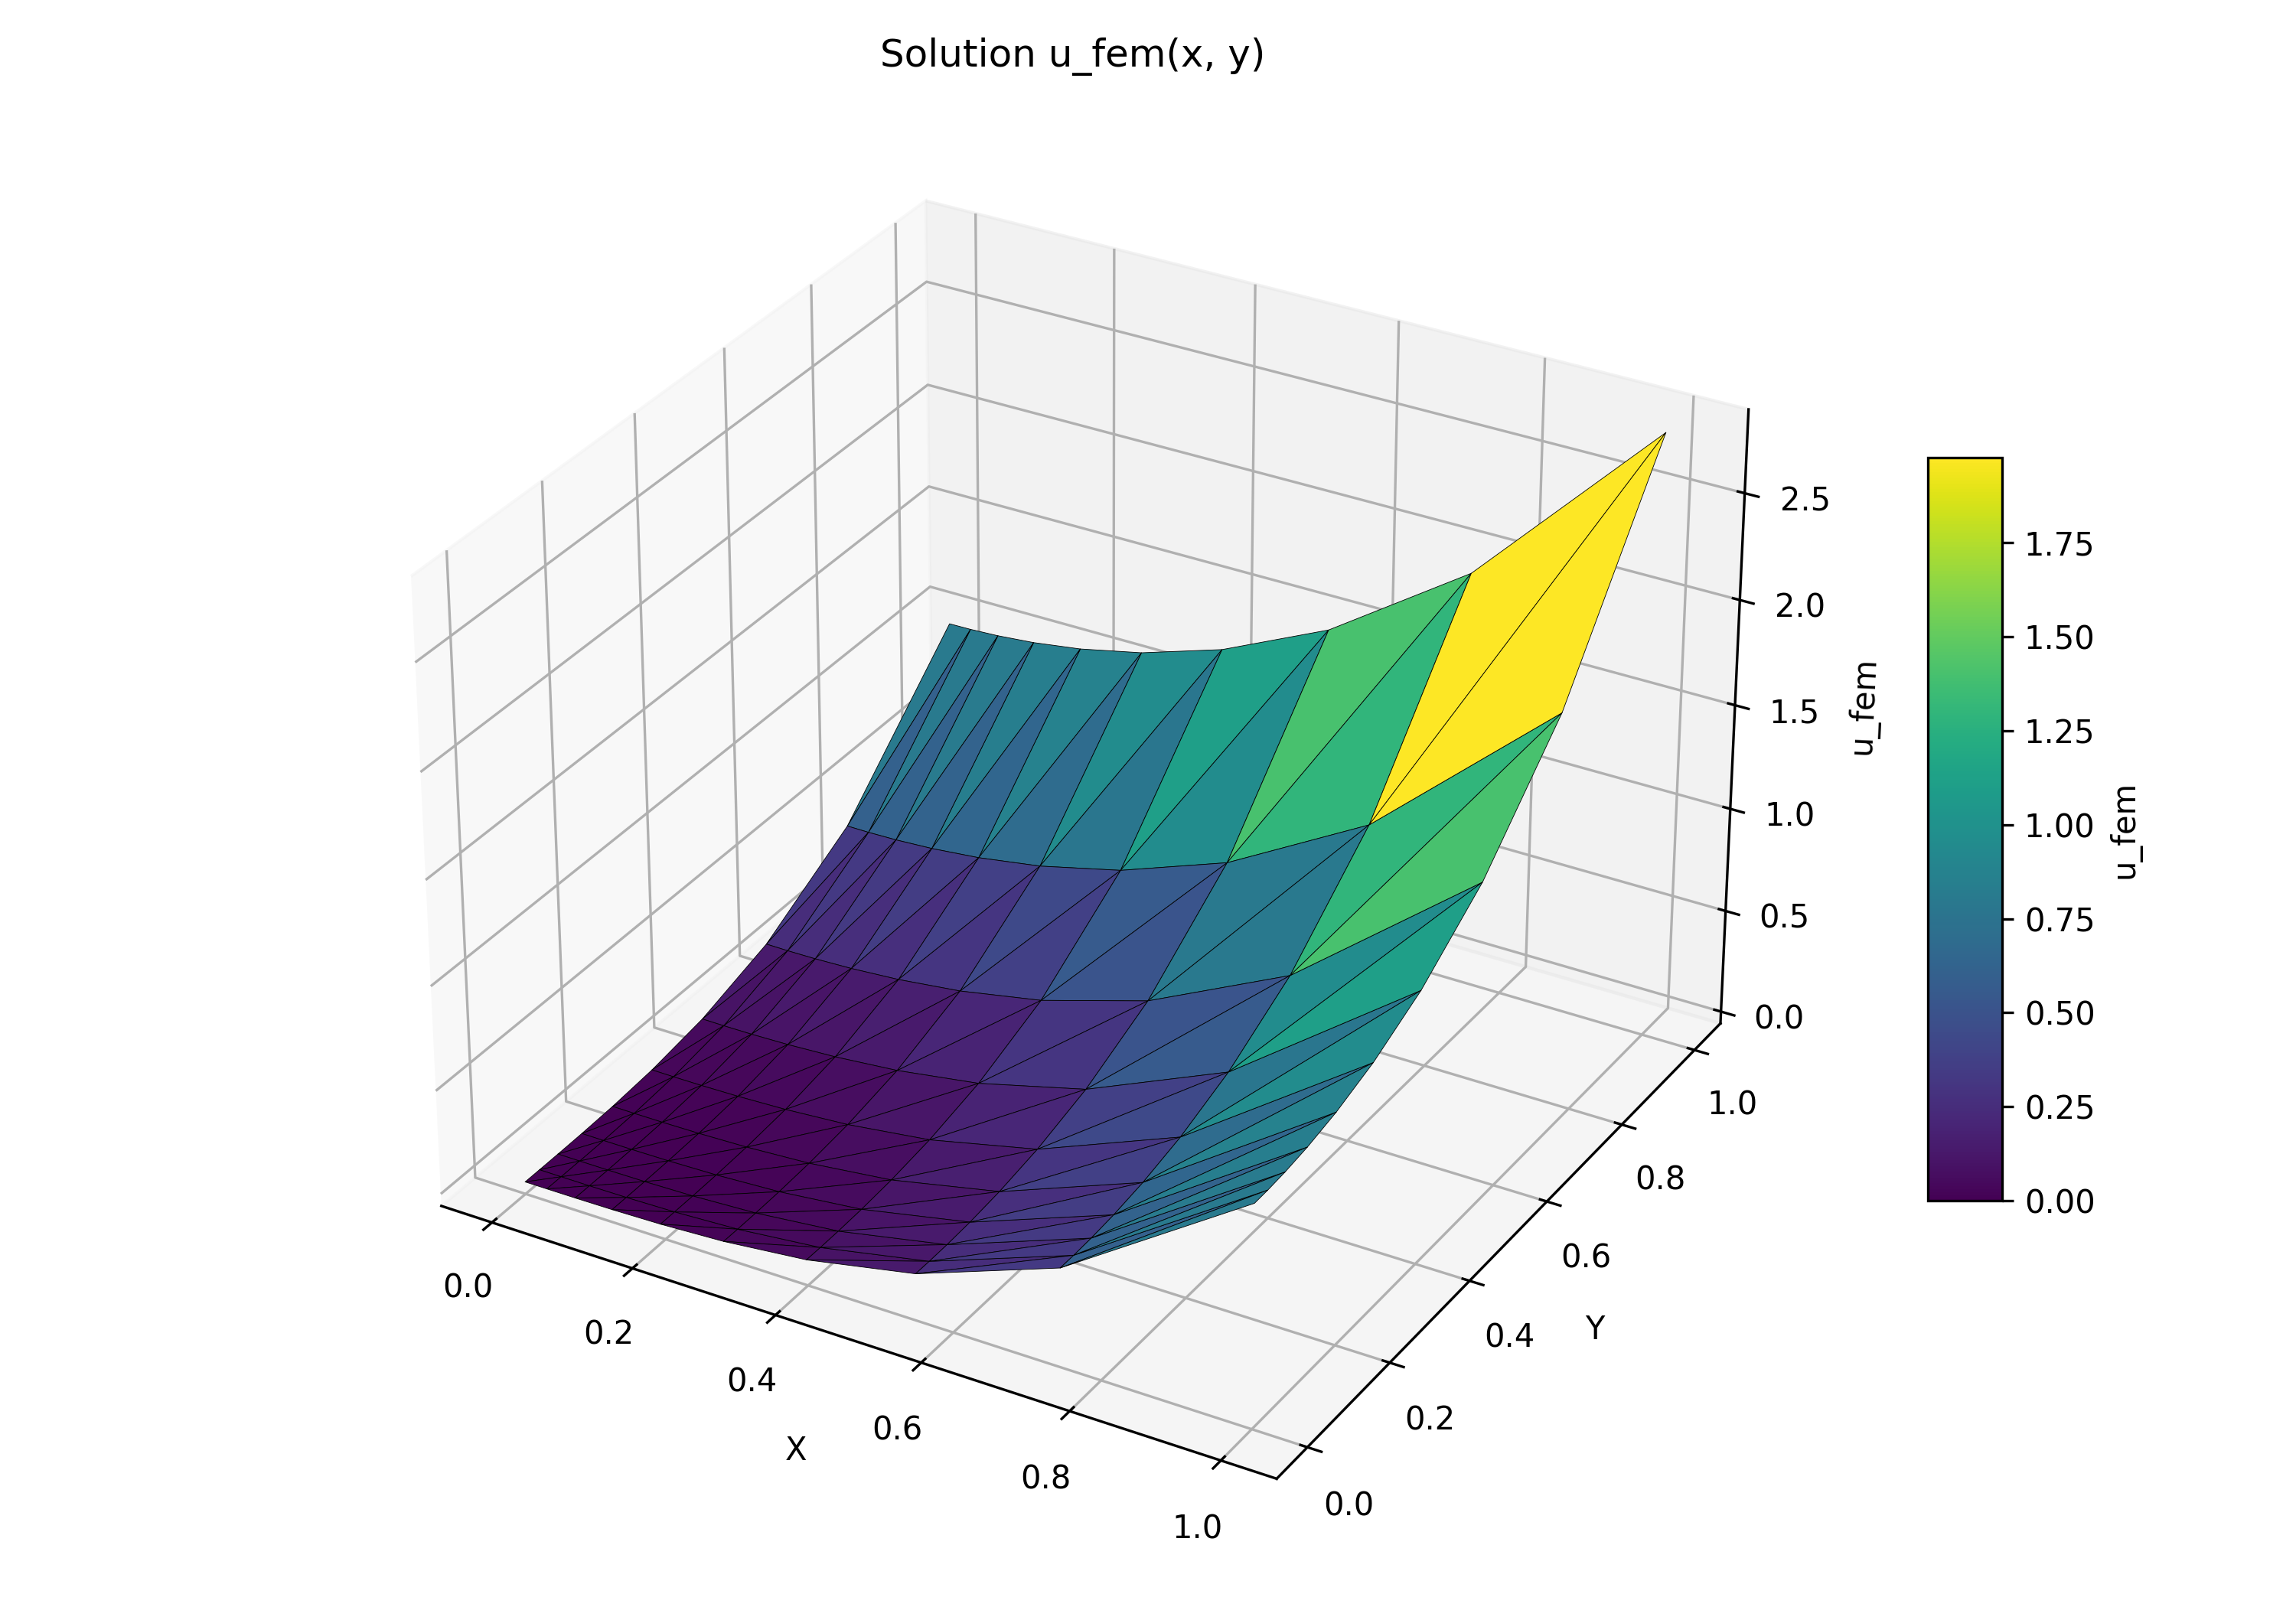
\includegraphics[width=\textwidth]{GRAFICOS/CST/CST_u_fem_sol_surface_plot.png}
    \caption{Discrete solution \(u_h\) for CST}
    \label{fig:cst_u_fem_sol}
  \end{subfigure}
  \hfill
  \begin{subfigure}[b]{0.48\textwidth}
    \centering
    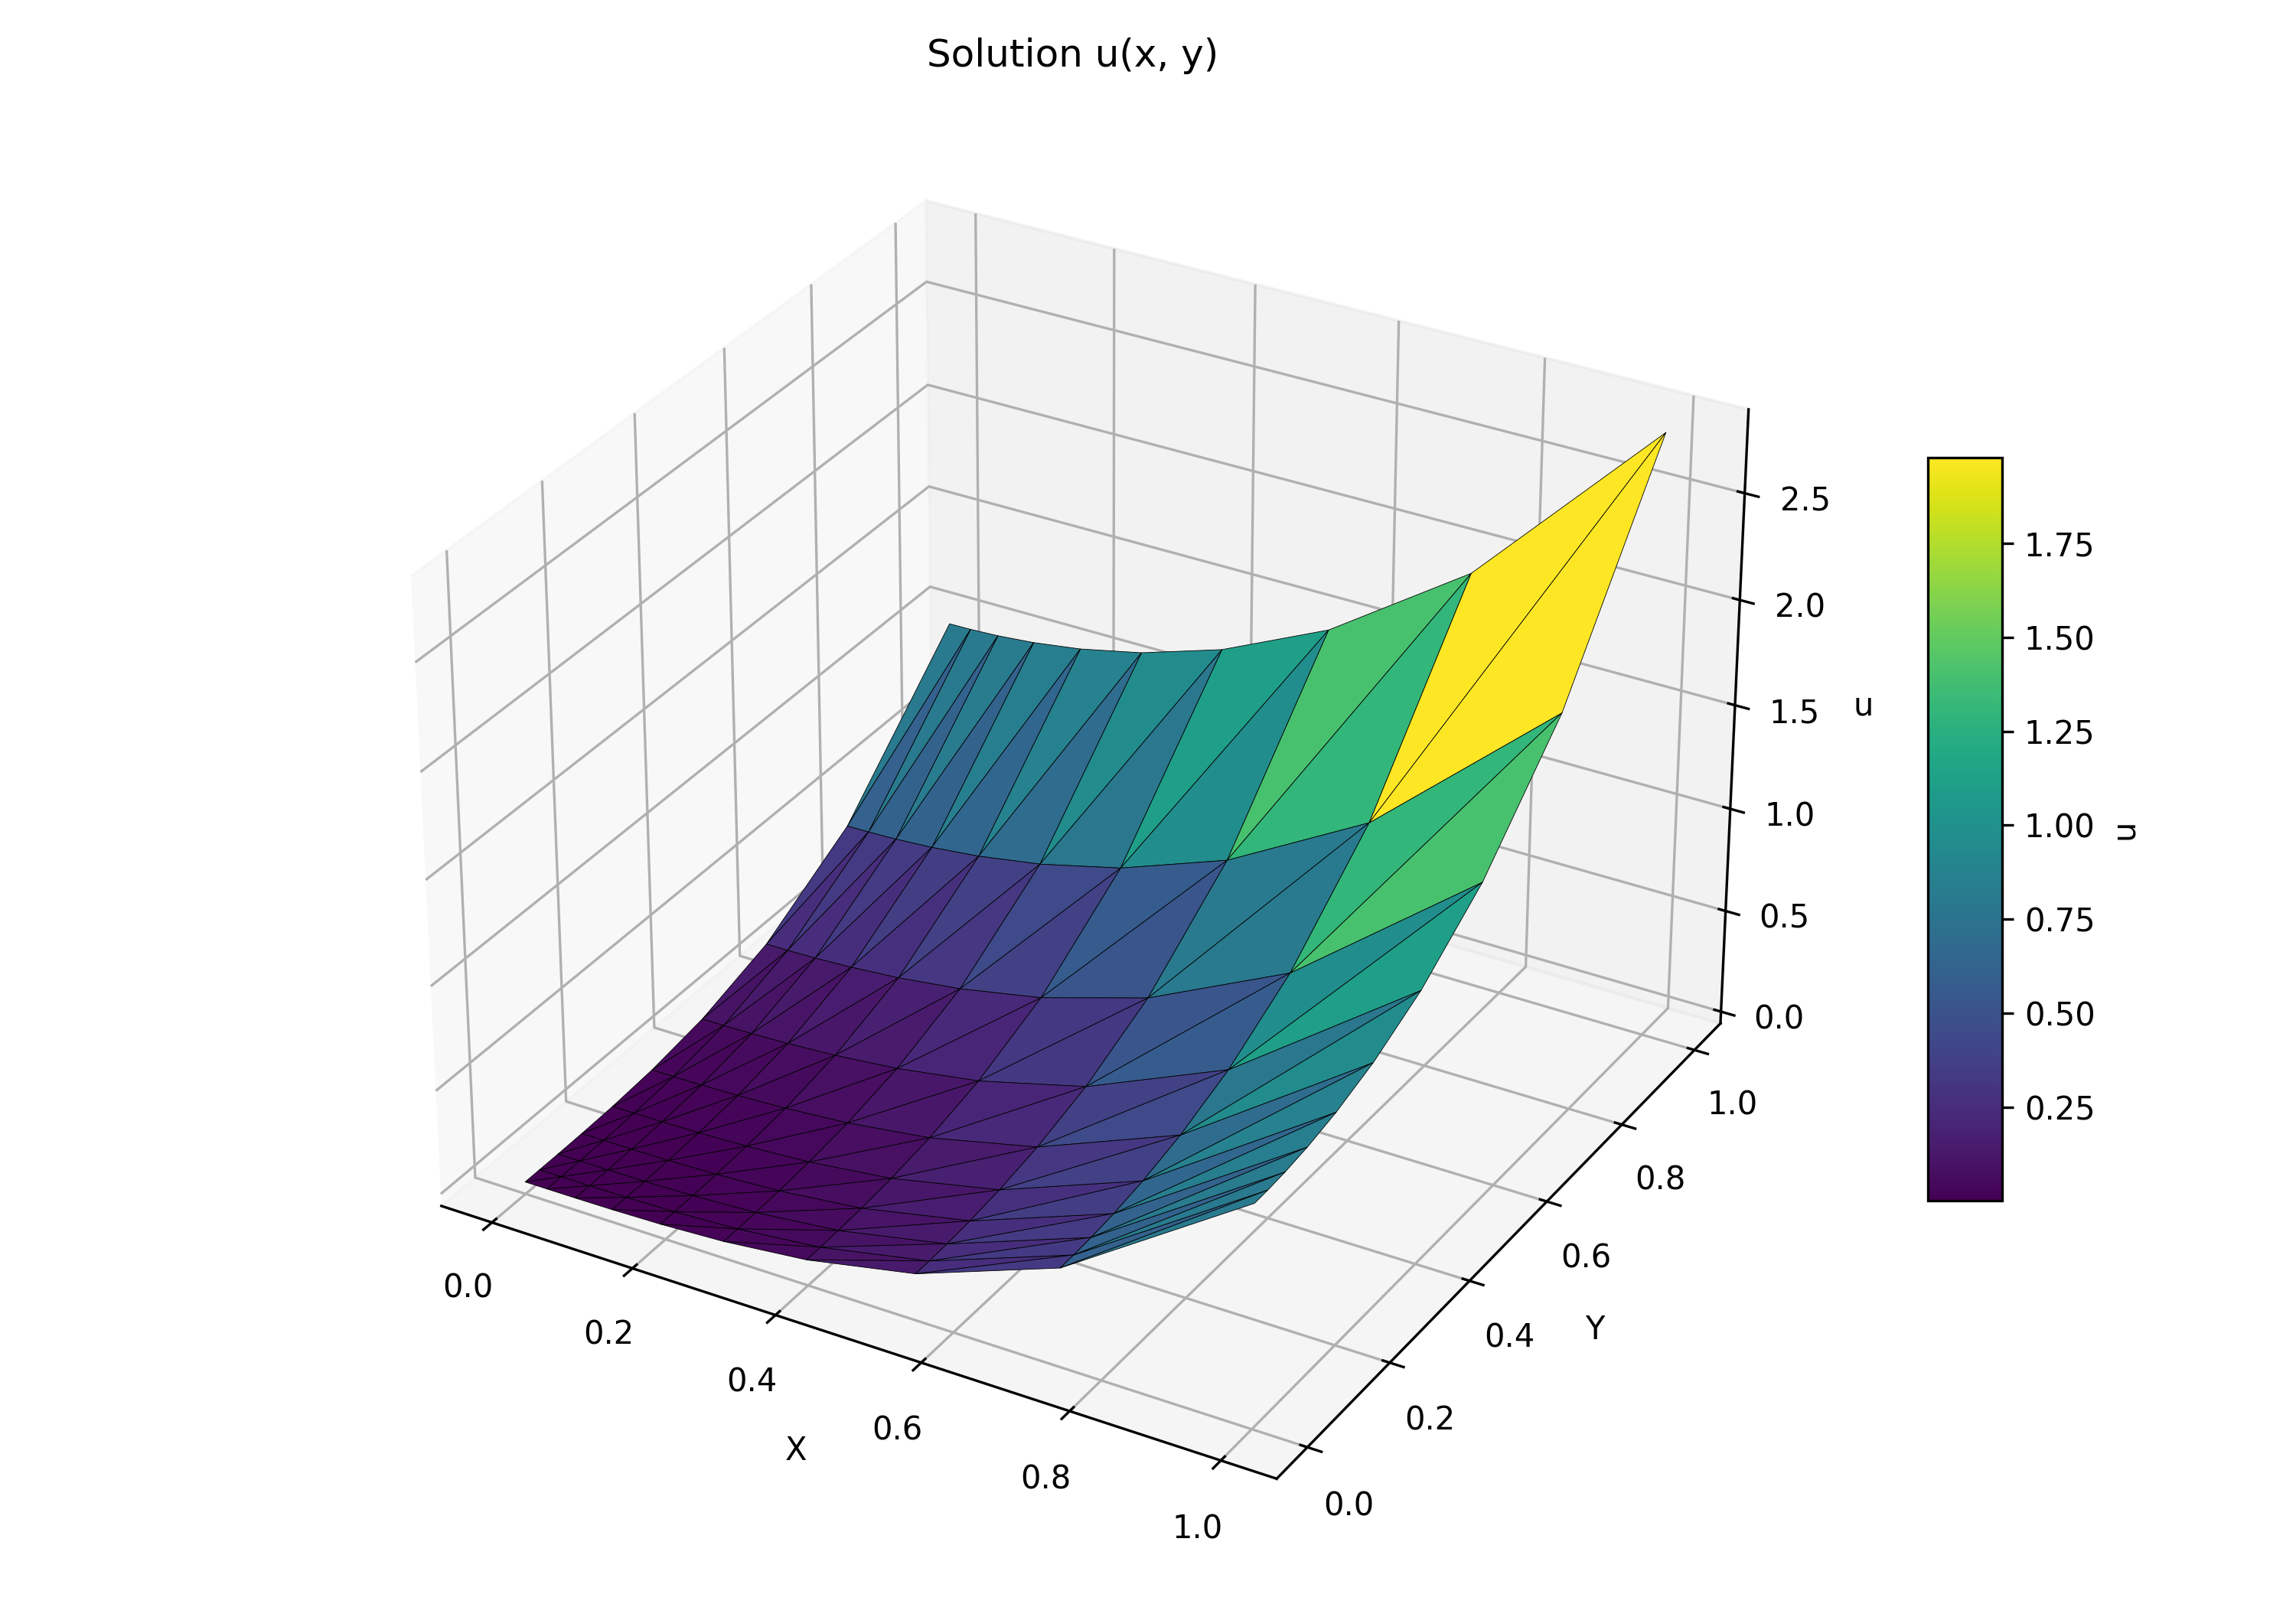
\includegraphics[width=\textwidth]{GRAFICOS/CST/CST_u_sol_surface_plot.png}
    \caption{Analytic solution \(u\) for CST}
    \label{fig:cst_error_plot}
  \end{subfigure}
  \caption{Comparison of the finite‐element discrete solution \(u_h\) and the analytic solution \(u\) for CST elements.}
  \label{fig:cst_comparison}
\end{figure}

\begin{figure}[H]
\centering
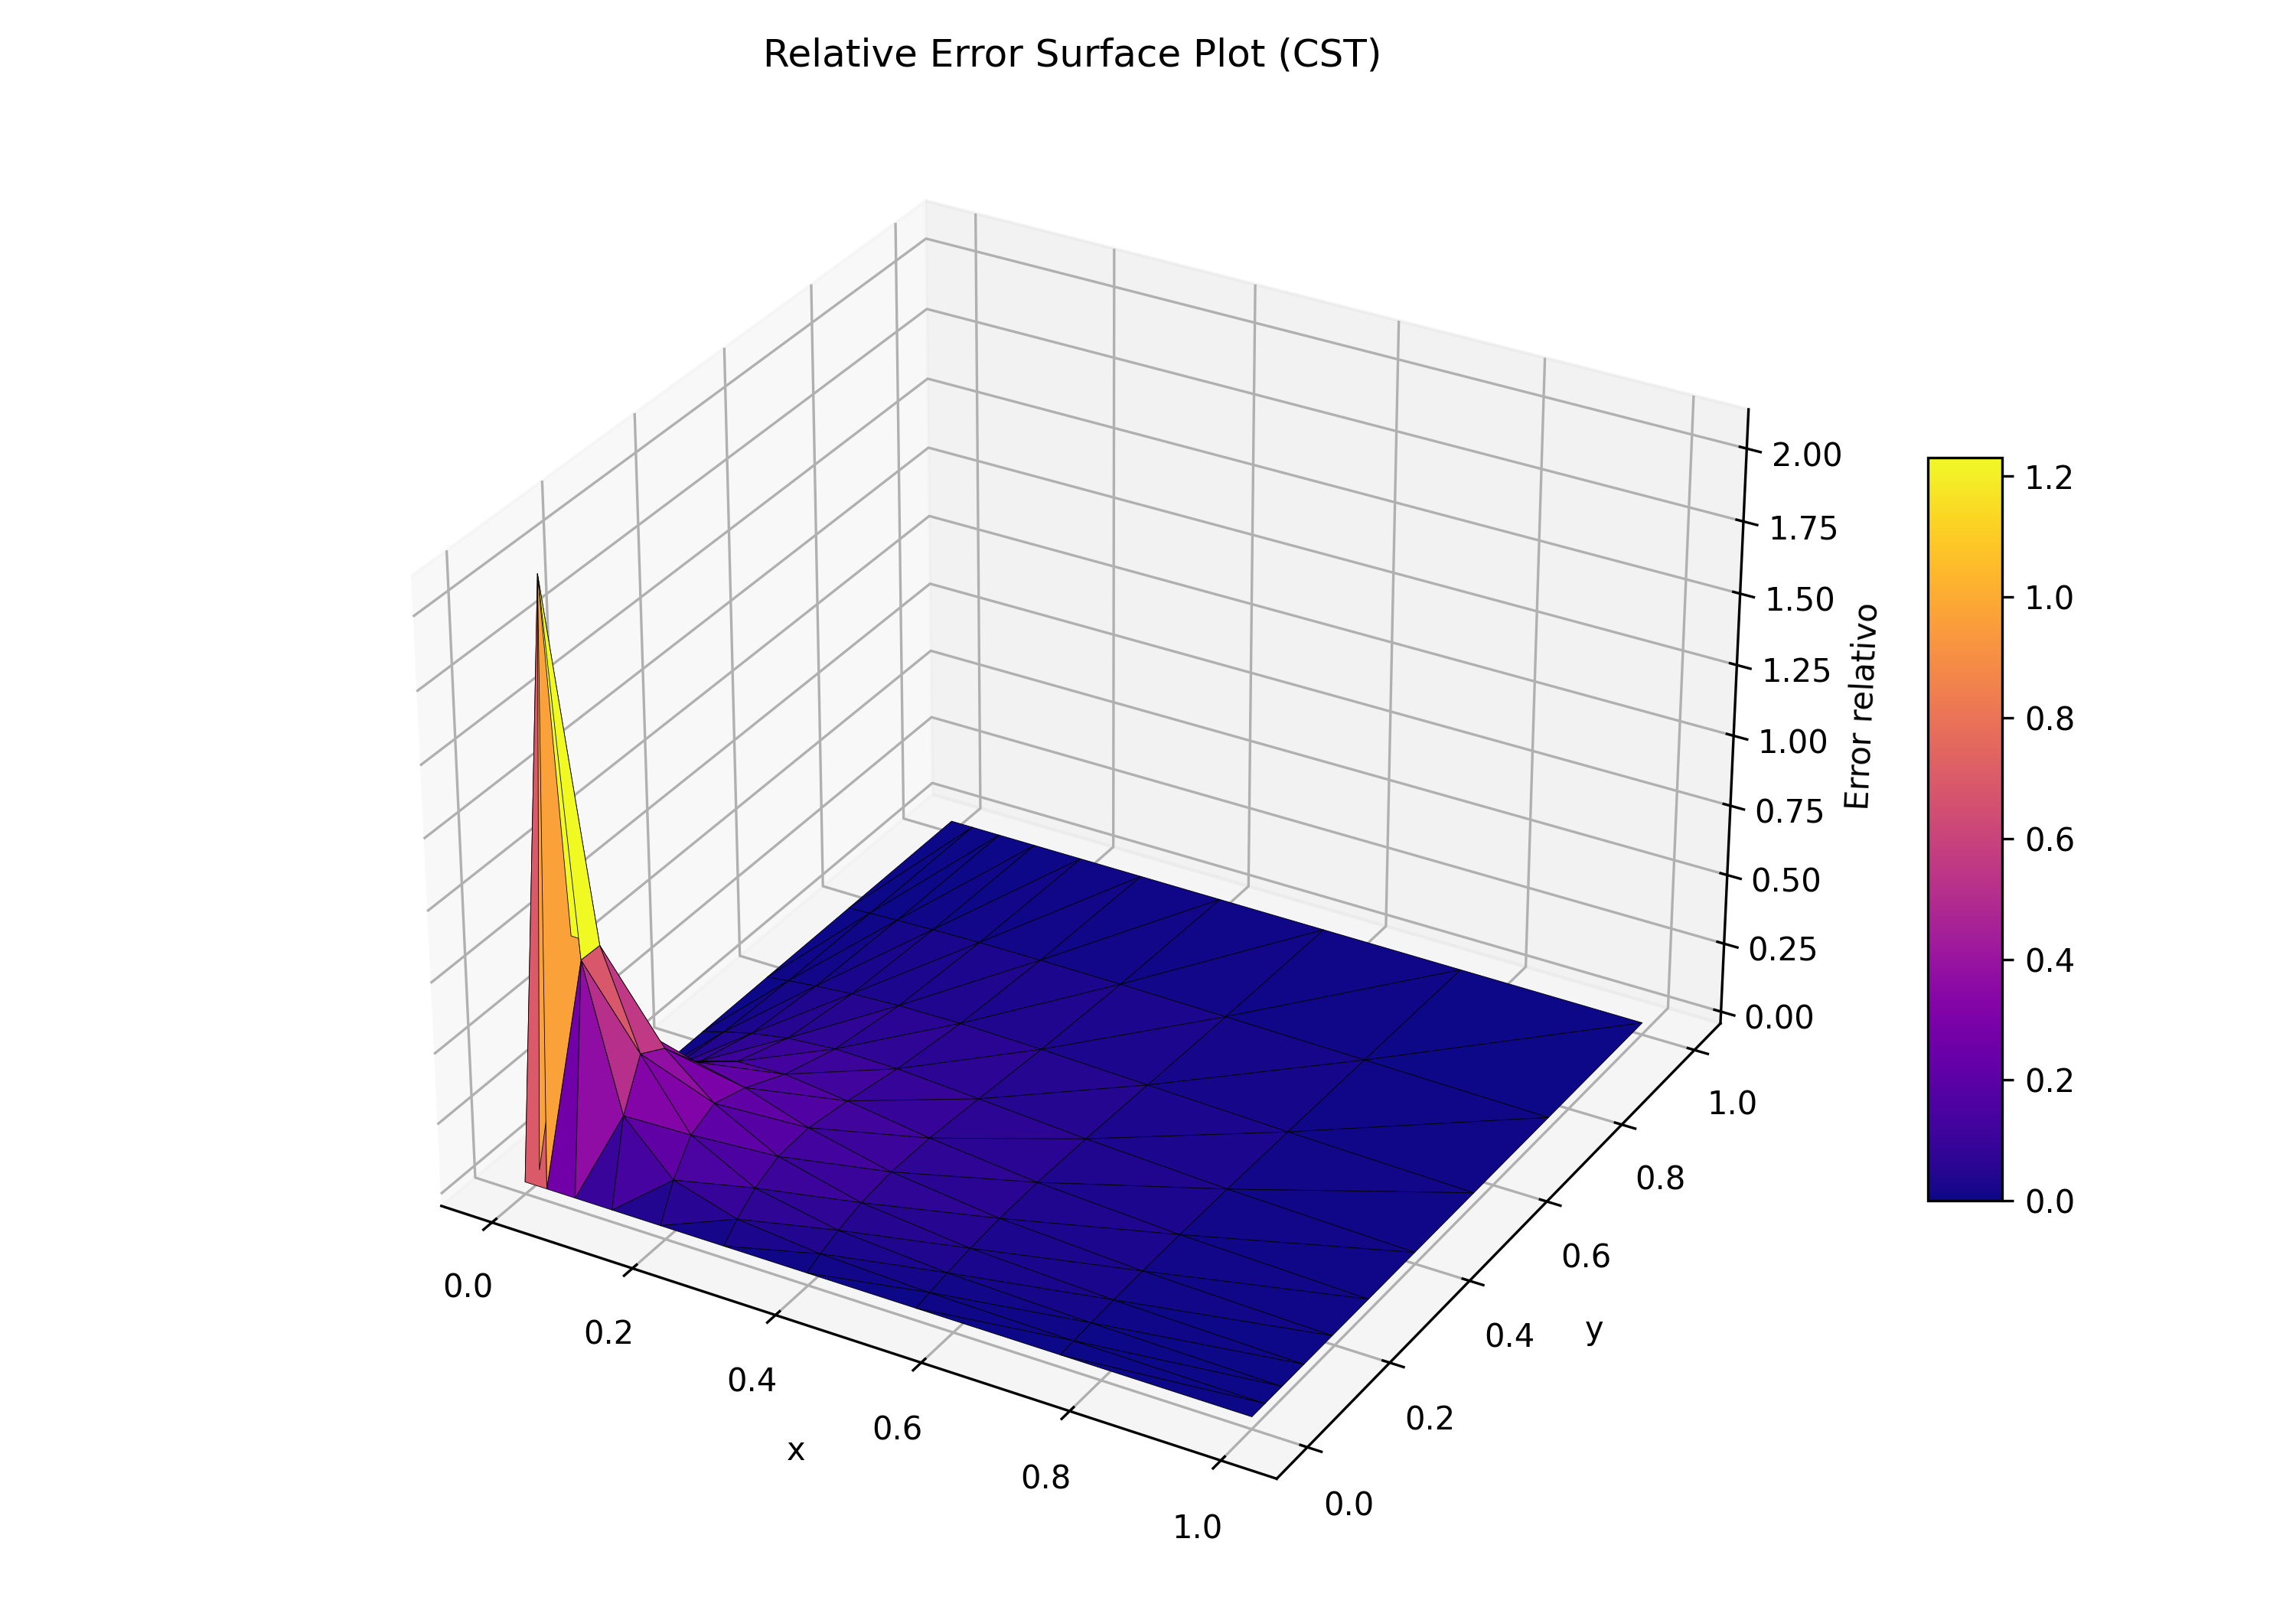
\includegraphics[width=0.6\textwidth]{GRAFICOS/CST/CST_relative_error_surface_plot.png}
\caption{Relative error \(\|u - u_h\|_{H^1(\Omega)}\) for CST elements}
\label{fig:cst_error_vs_h}
\end{figure}

\begin{figure}[H]
\centering
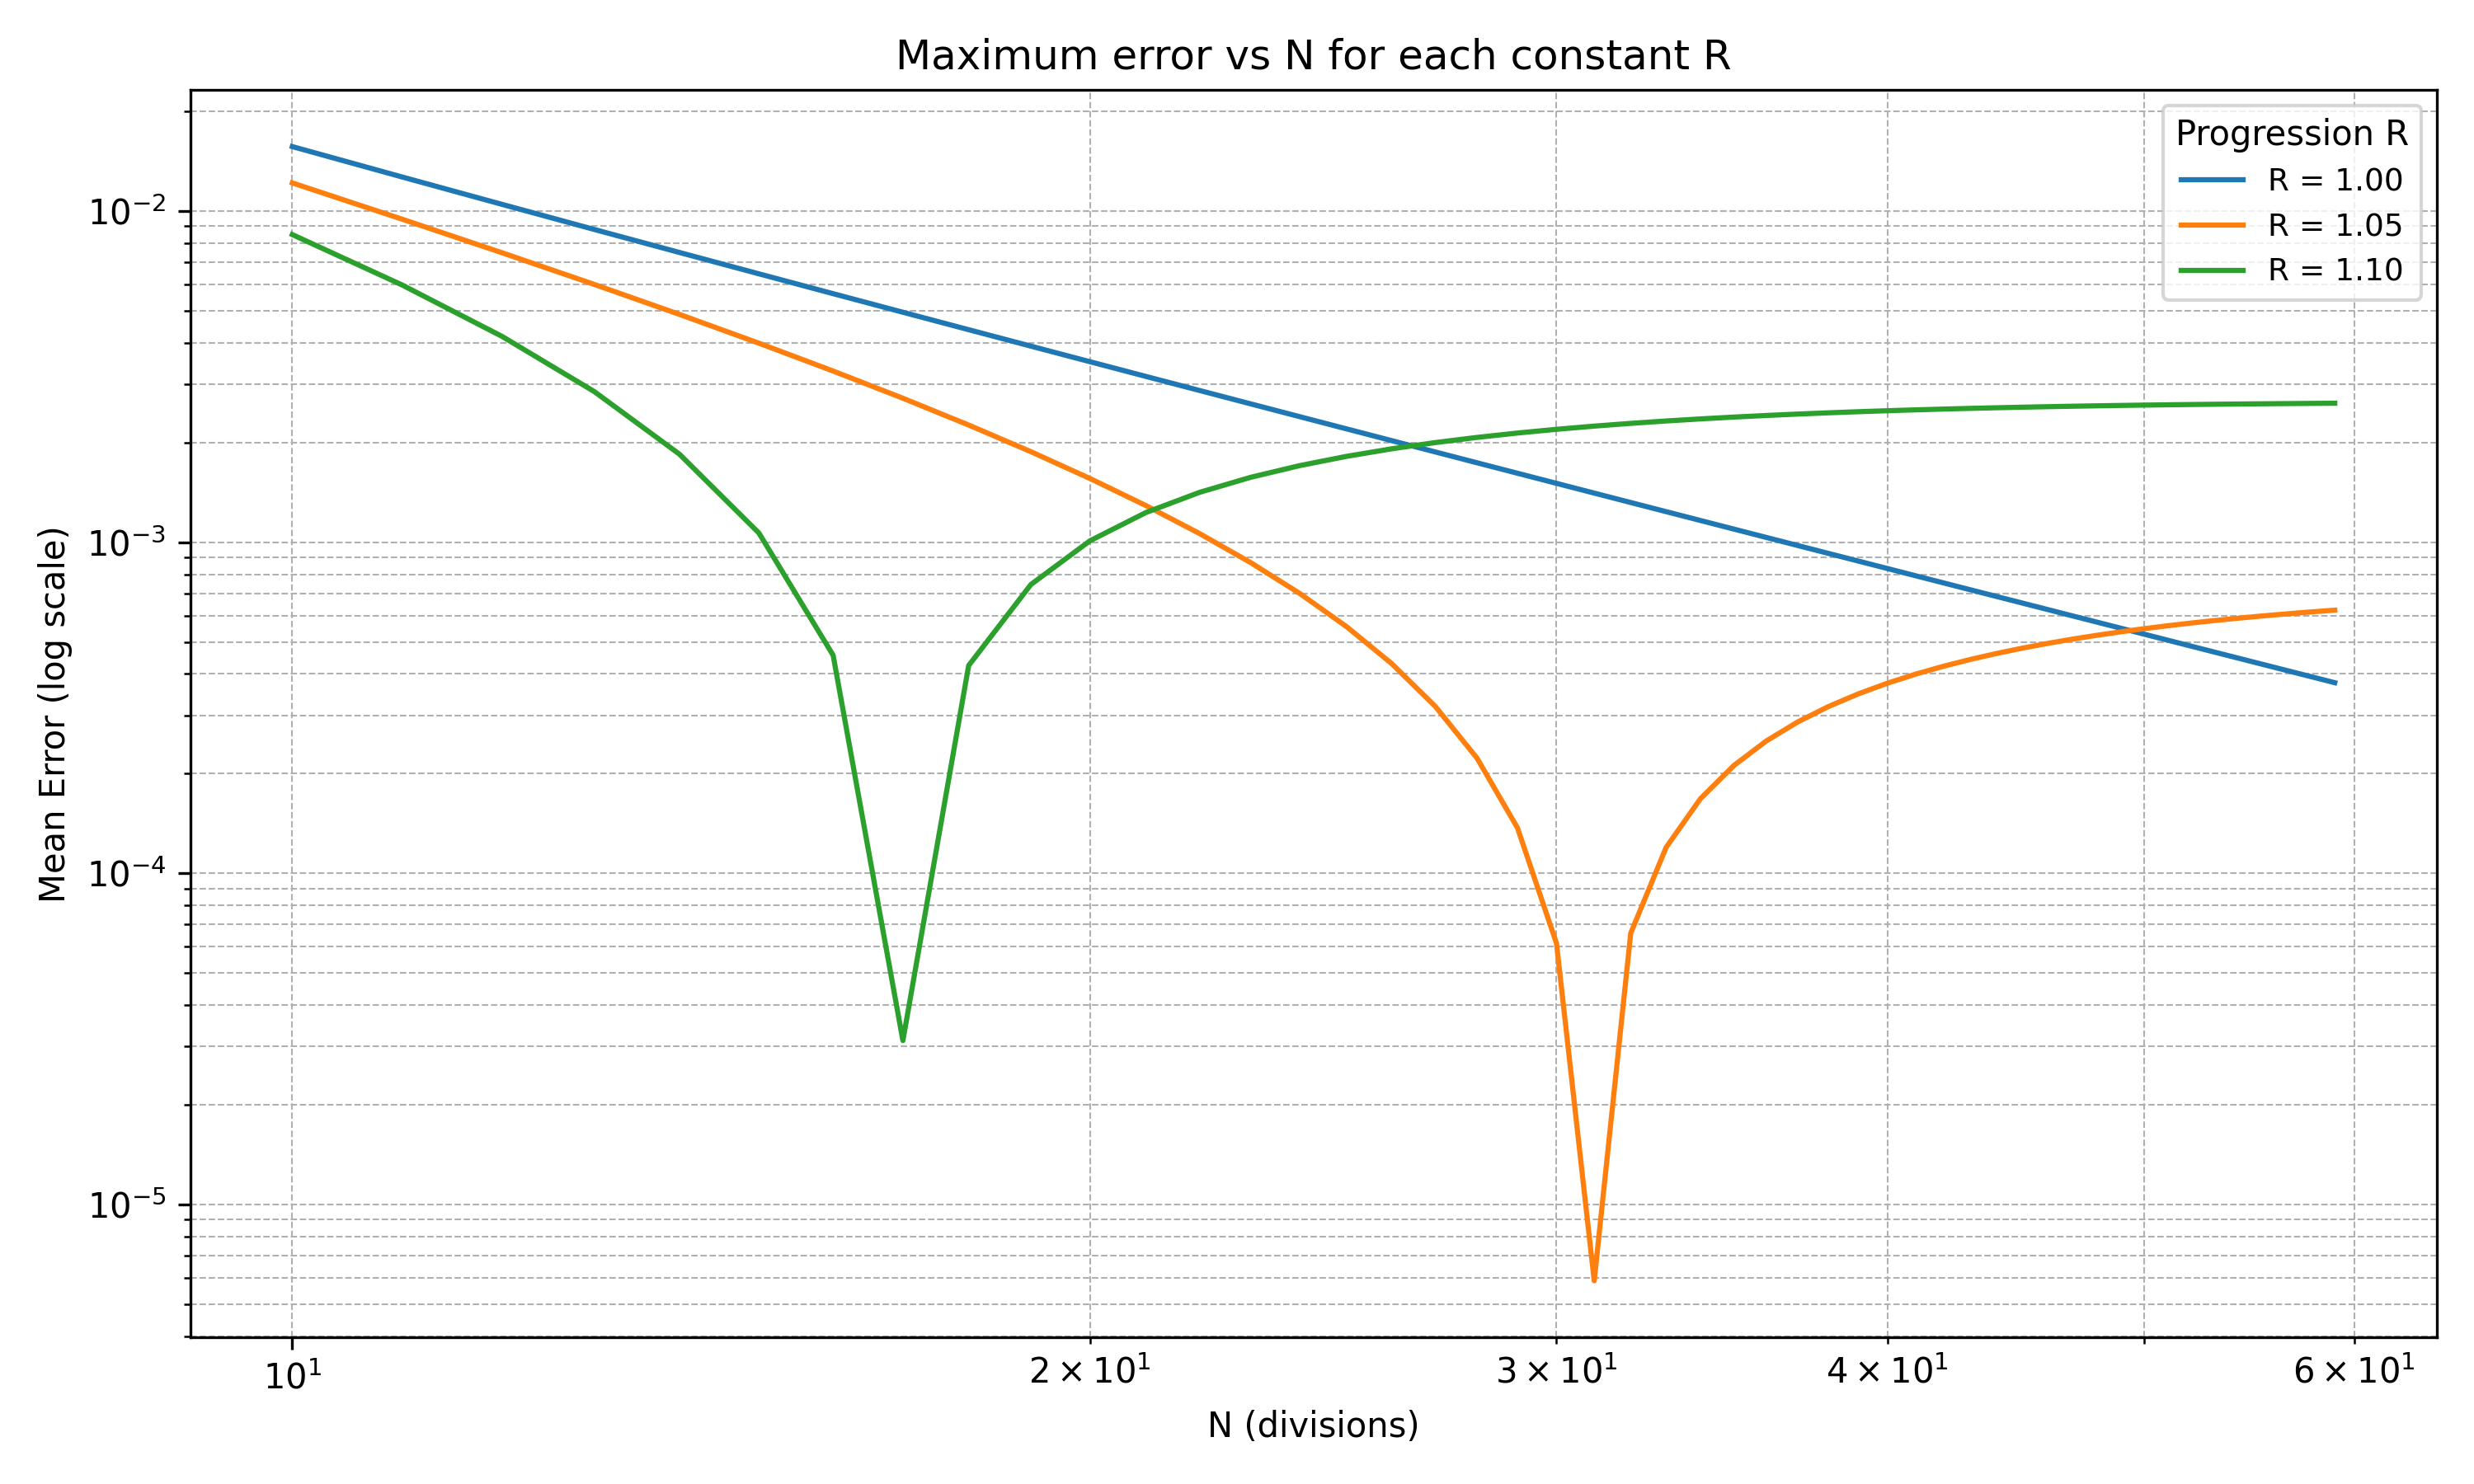
\includegraphics[width=0.6\textwidth]{GRAFICOS/CST/errores_por_R.png}
\caption{Relative error \(\|u - u_h\|_{H^1(\Omega)}\) with varying progression parameter $r$ and $N$ divisions of the mesh for CST elements.}
\label{fig:cst_error_vs_h_loglog}
\end{figure}

Figure \ref{fig:cst_comparison} shows the comparison between the discrete solution using Guassian Quadrature ($u_H$) and the analytic solution ($u$) using finite element method, for CST elements. Both solutions reach values close to 2.5, thus the relative error in Figure \ref{fig:cst_error_vs_h} is almost 0, this was the result of substracting both solutions as \(\|u - u_h\|_{H^1(\Omega)}\). The singularity observed in this plot is due to the indefinition of the derivatives close to the Dirichlet point $(0,0)$. 

Moreover, the relative error in Figure \ref{fig:cst_error_vs_h_loglog} shows the convergence of the method, as the mesh is refined, increasing the number of elements $(N-1)^2$, the error decreases and converges to 0. 

\subsection{LST annalysis}

\begin{figure}[H]
\centering
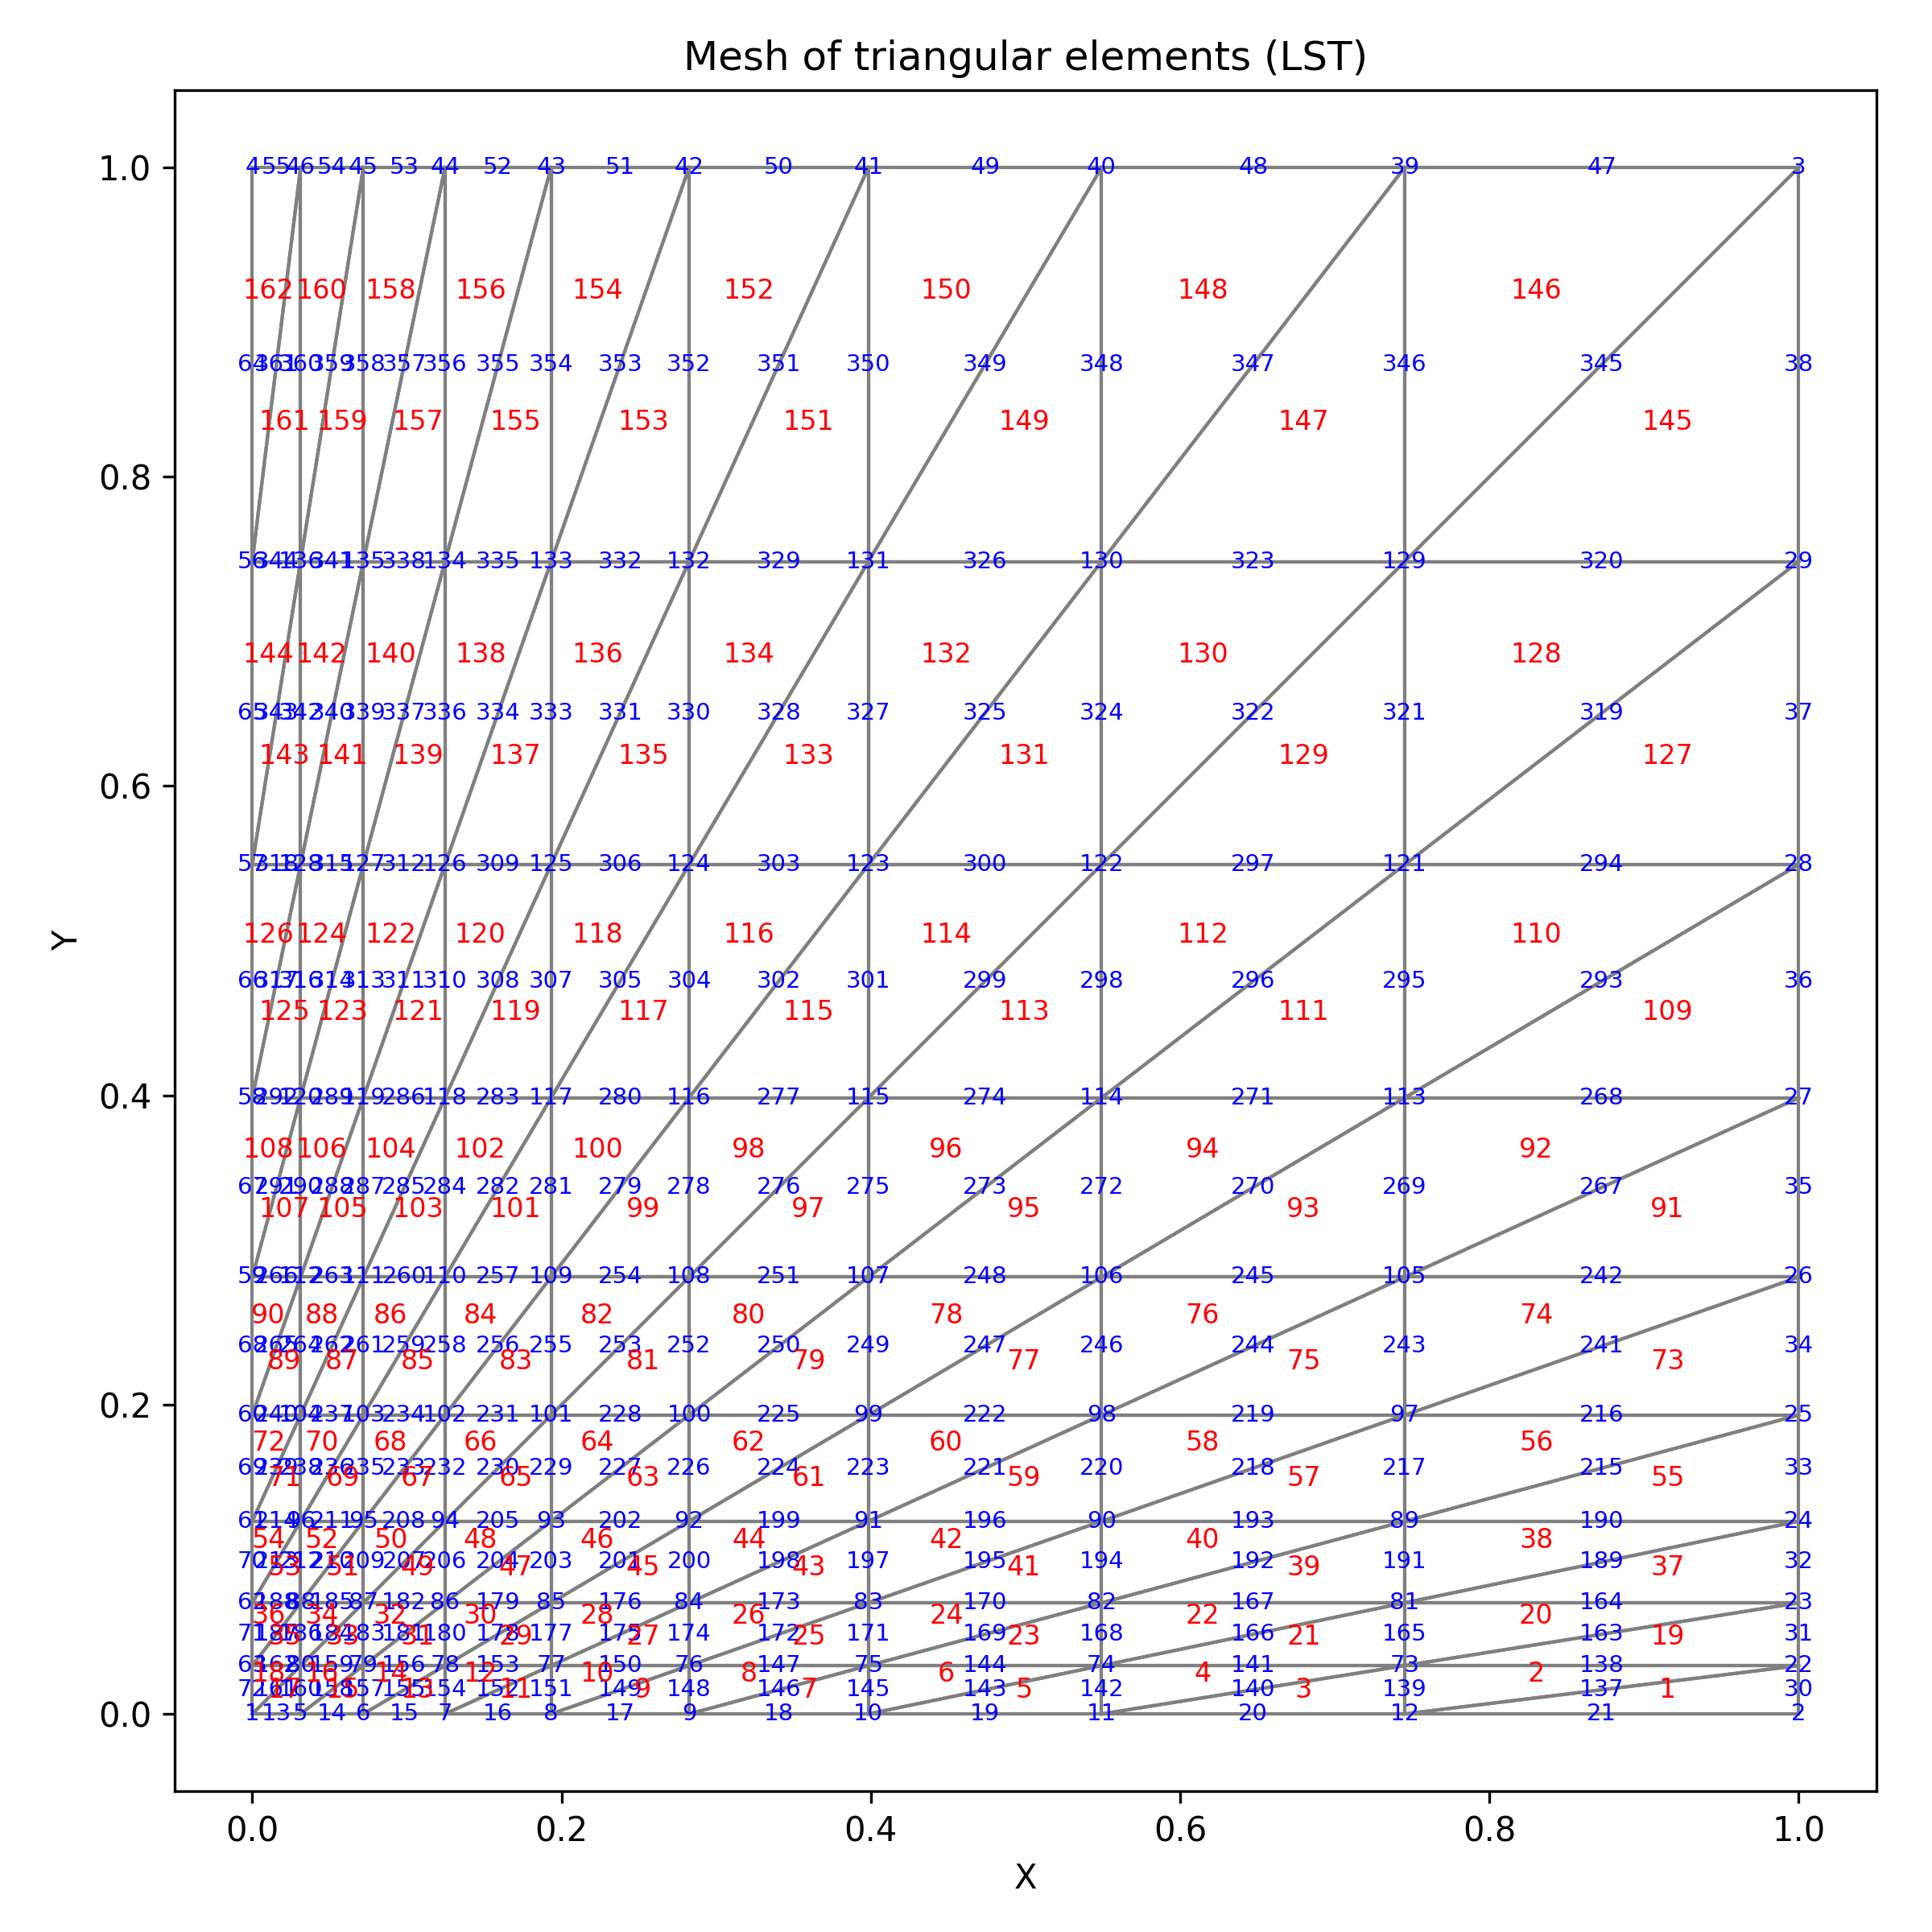
\includegraphics[width=0.4\textwidth]{GRAFICOS/LST/LST_mesh_plot.png}
\caption{LST Mesh}
\label{fig:lst_results}
\end{figure}

\begin{figure}[H]
\centering
\begin{subfigure}[b]{0.48\textwidth}
    \centering
    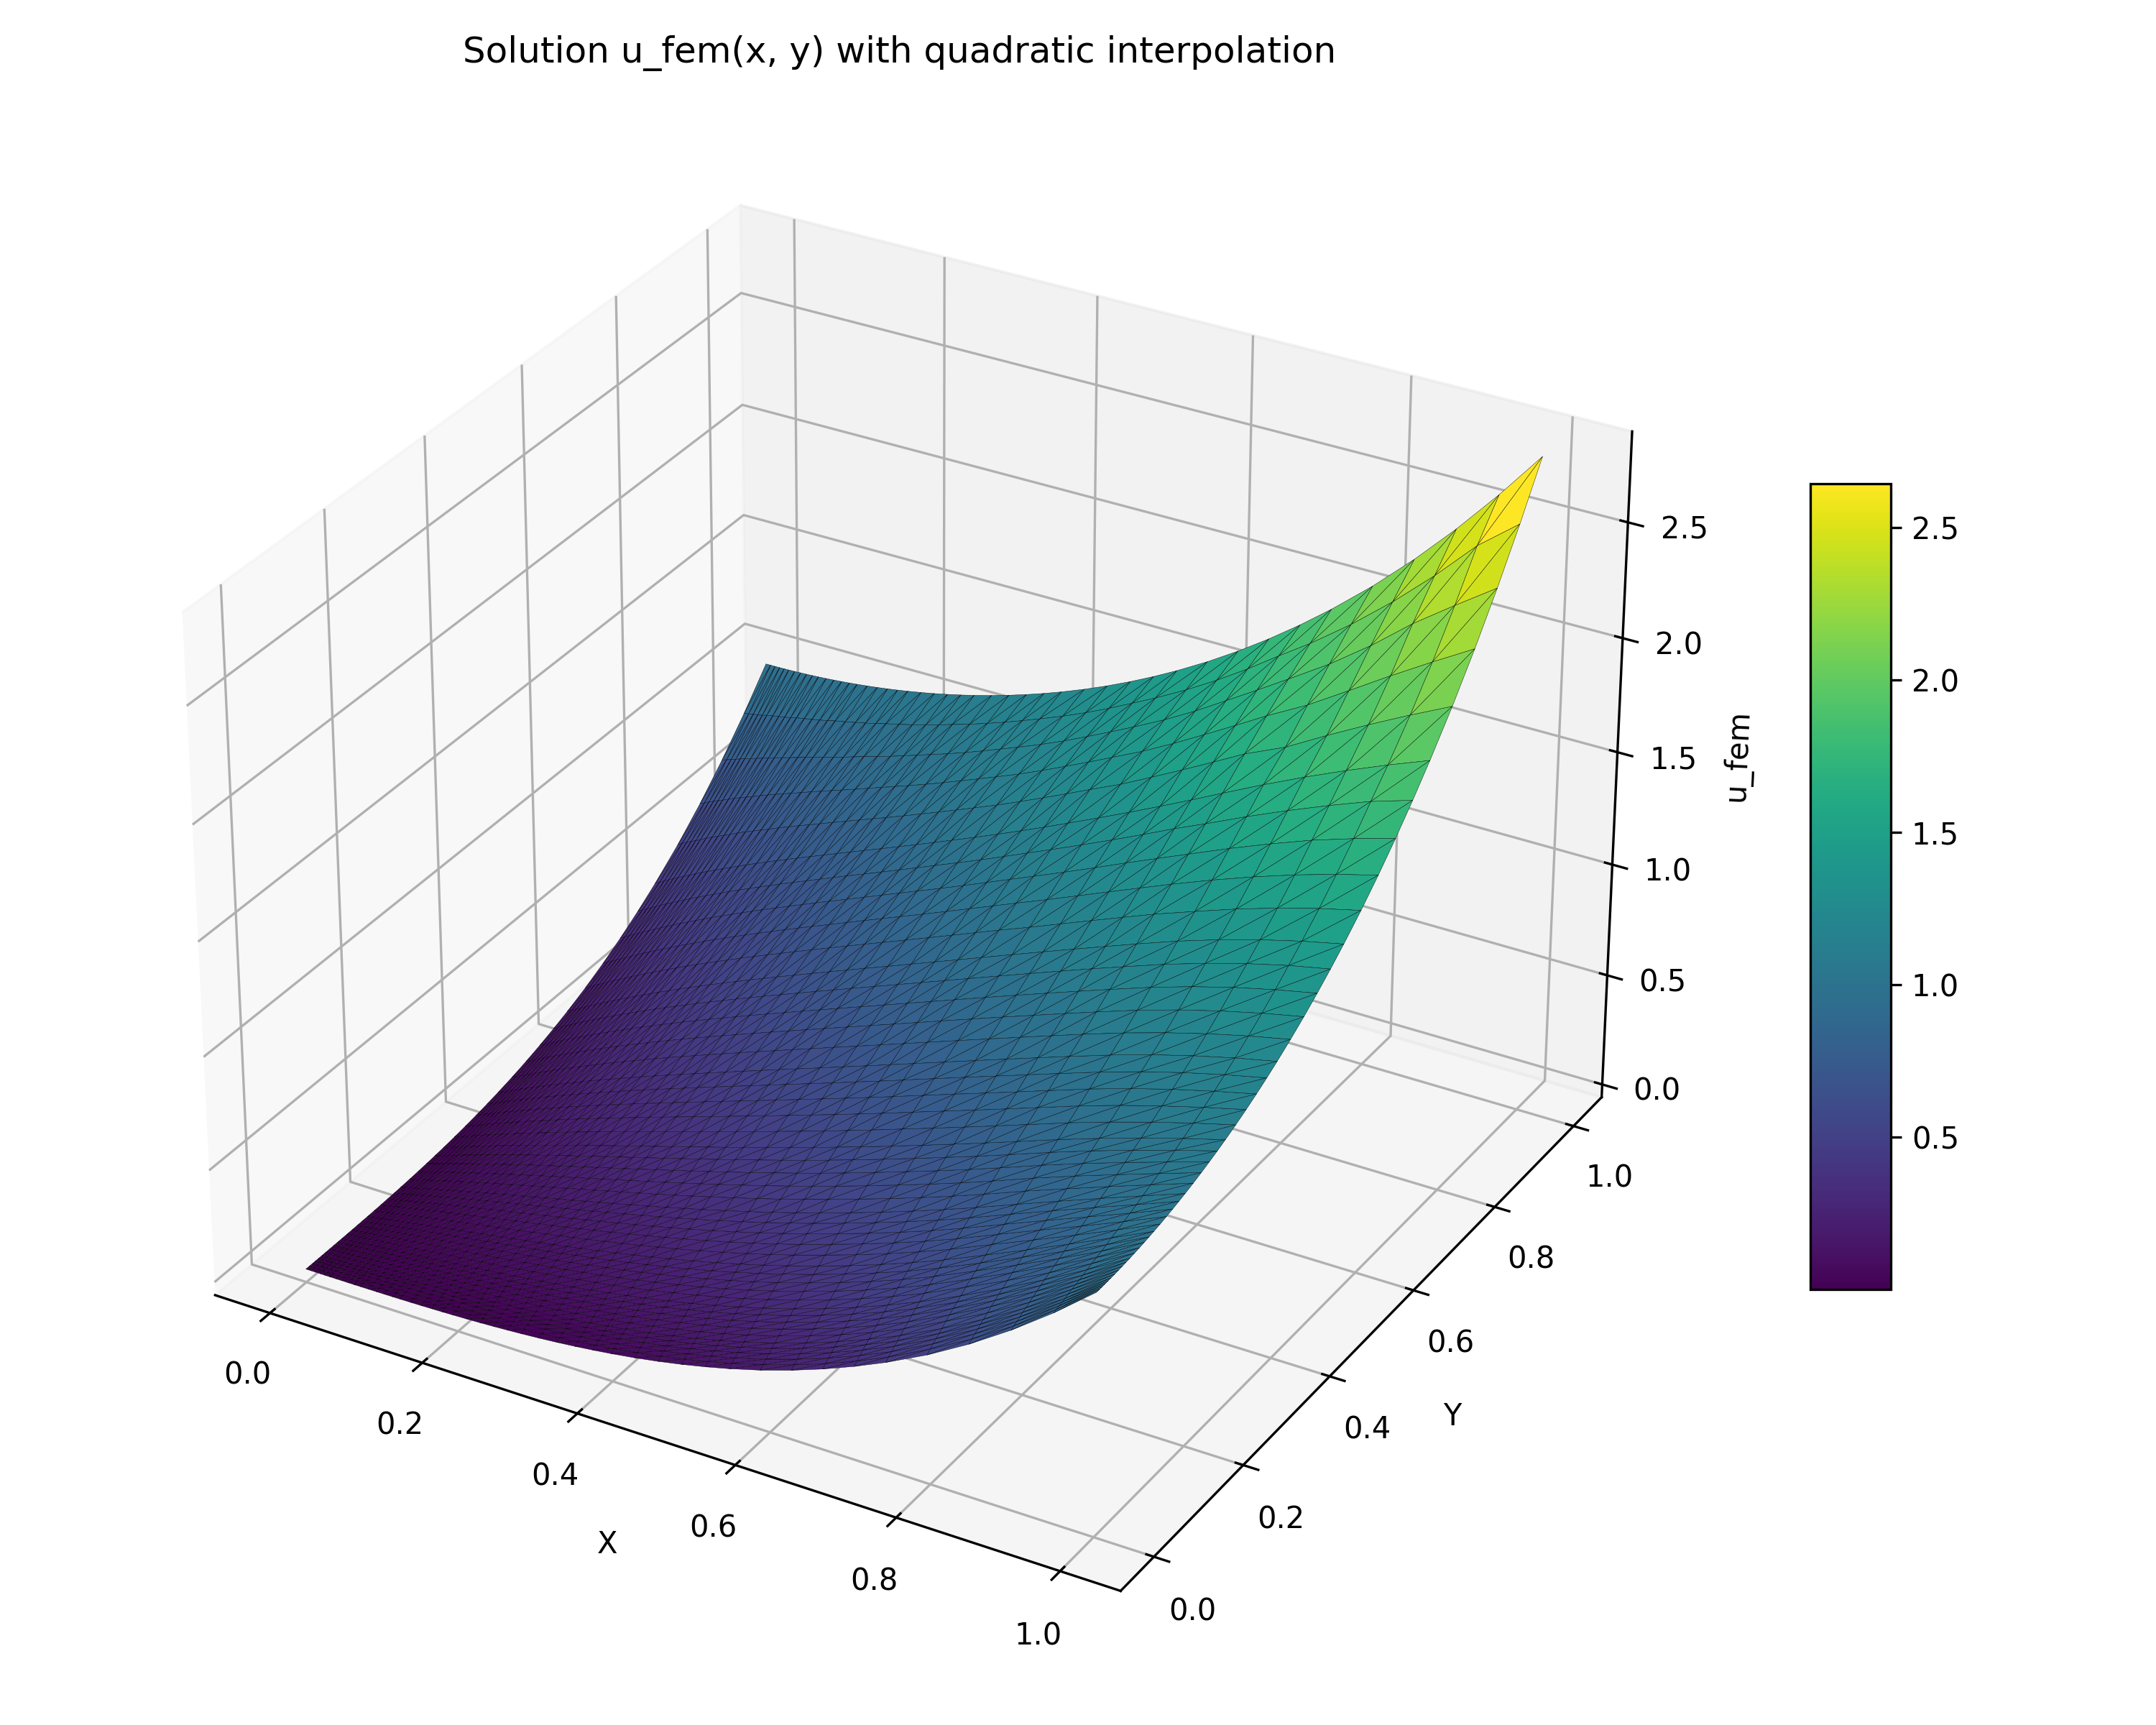
\includegraphics[width=\textwidth]{GRAFICOS/LST/LST_u_fem_sol_surface_plot.png}
    \caption{Discrete solution \(u_h\) for LST}
    \label{fig:lst_u_fem_sol}
  \end{subfigure}
  \hfill
  \begin{subfigure}[b]{0.48\textwidth}
    \centering
    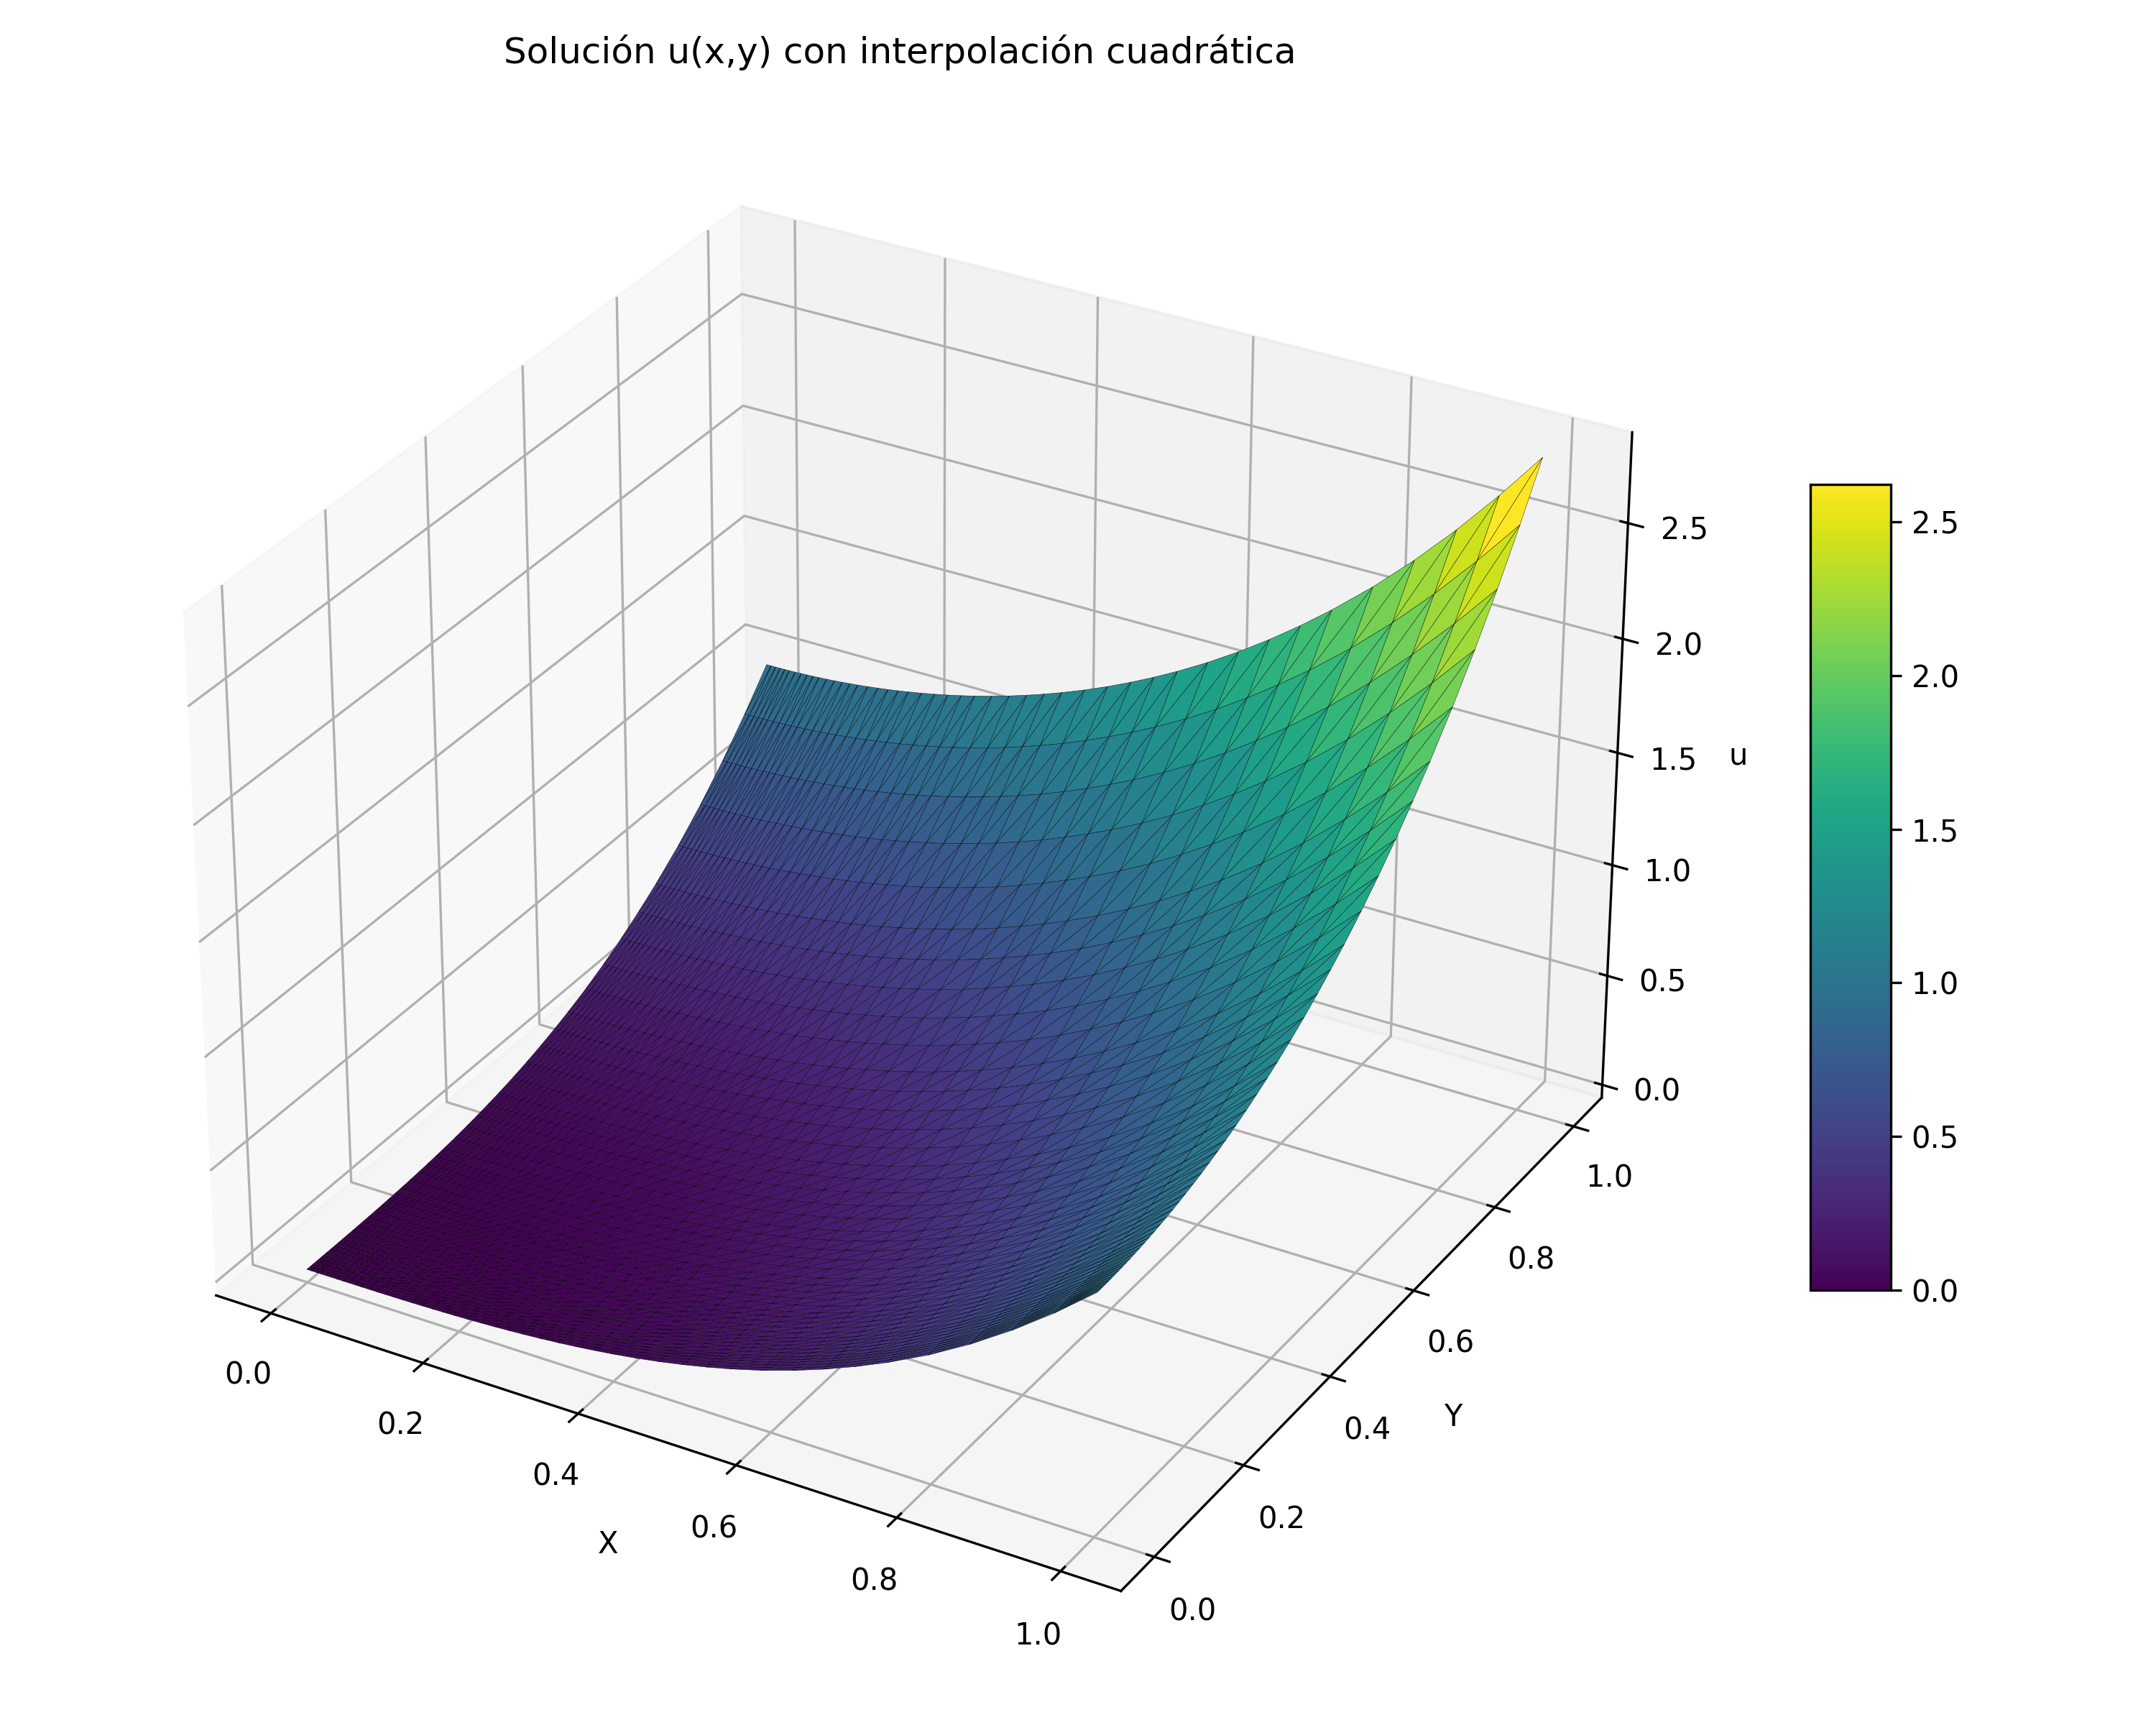
\includegraphics[width=\textwidth]{GRAFICOS/LST/LST_u_sol_surface_plot.png}
    \caption{Analytic solution \(u\) for LST}
    \label{fig:lst_error_plot}
  \end{subfigure}
  \caption{Comparison of the finite‐element discrete solution \(u_h\) and the analytic solution \(u\) for LST elements.}
  \label{fig:lst_comparison}
\end{figure}

\begin{figure}[H]
\centering
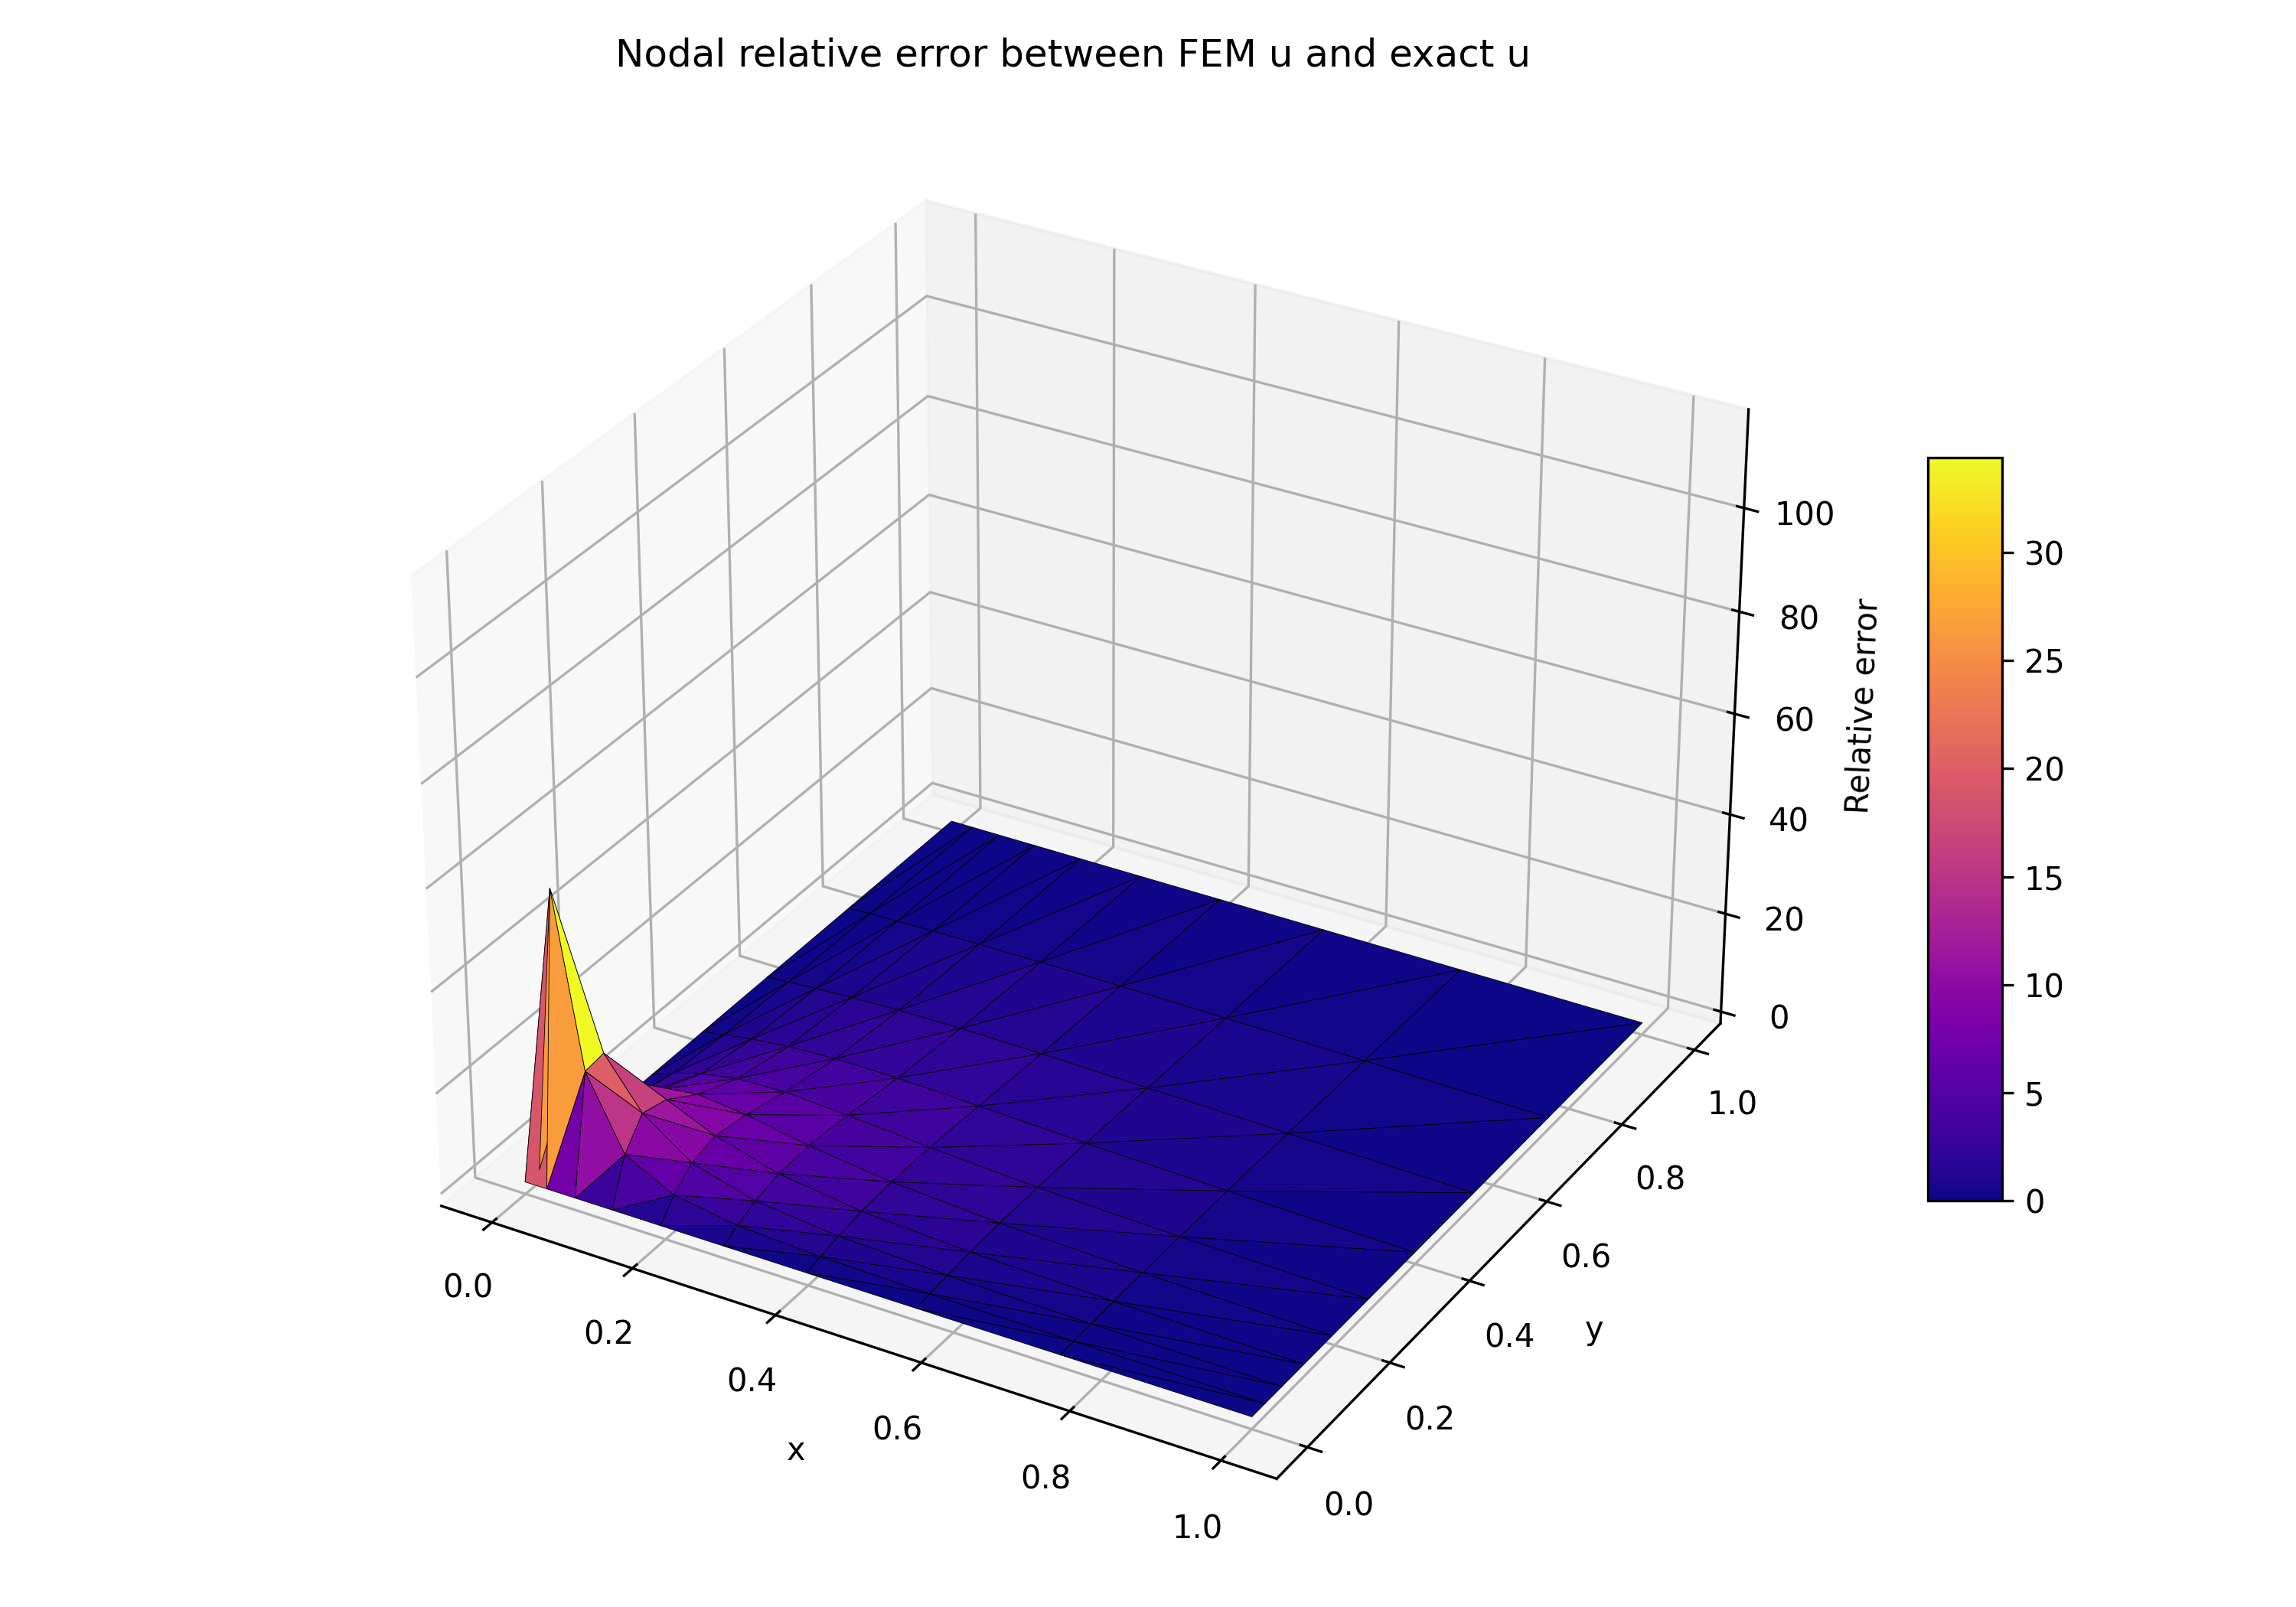
\includegraphics[width=0.6\textwidth]{GRAFICOS/LST/LST_relative_error_surface_plot.png}
\caption{Relative error \(\|u - u_h\|_{H^1(\Omega)}\) for LST elements}
\label{fig:lst_error_vs_h}
\end{figure}

\begin{figure}[H]
\centering 
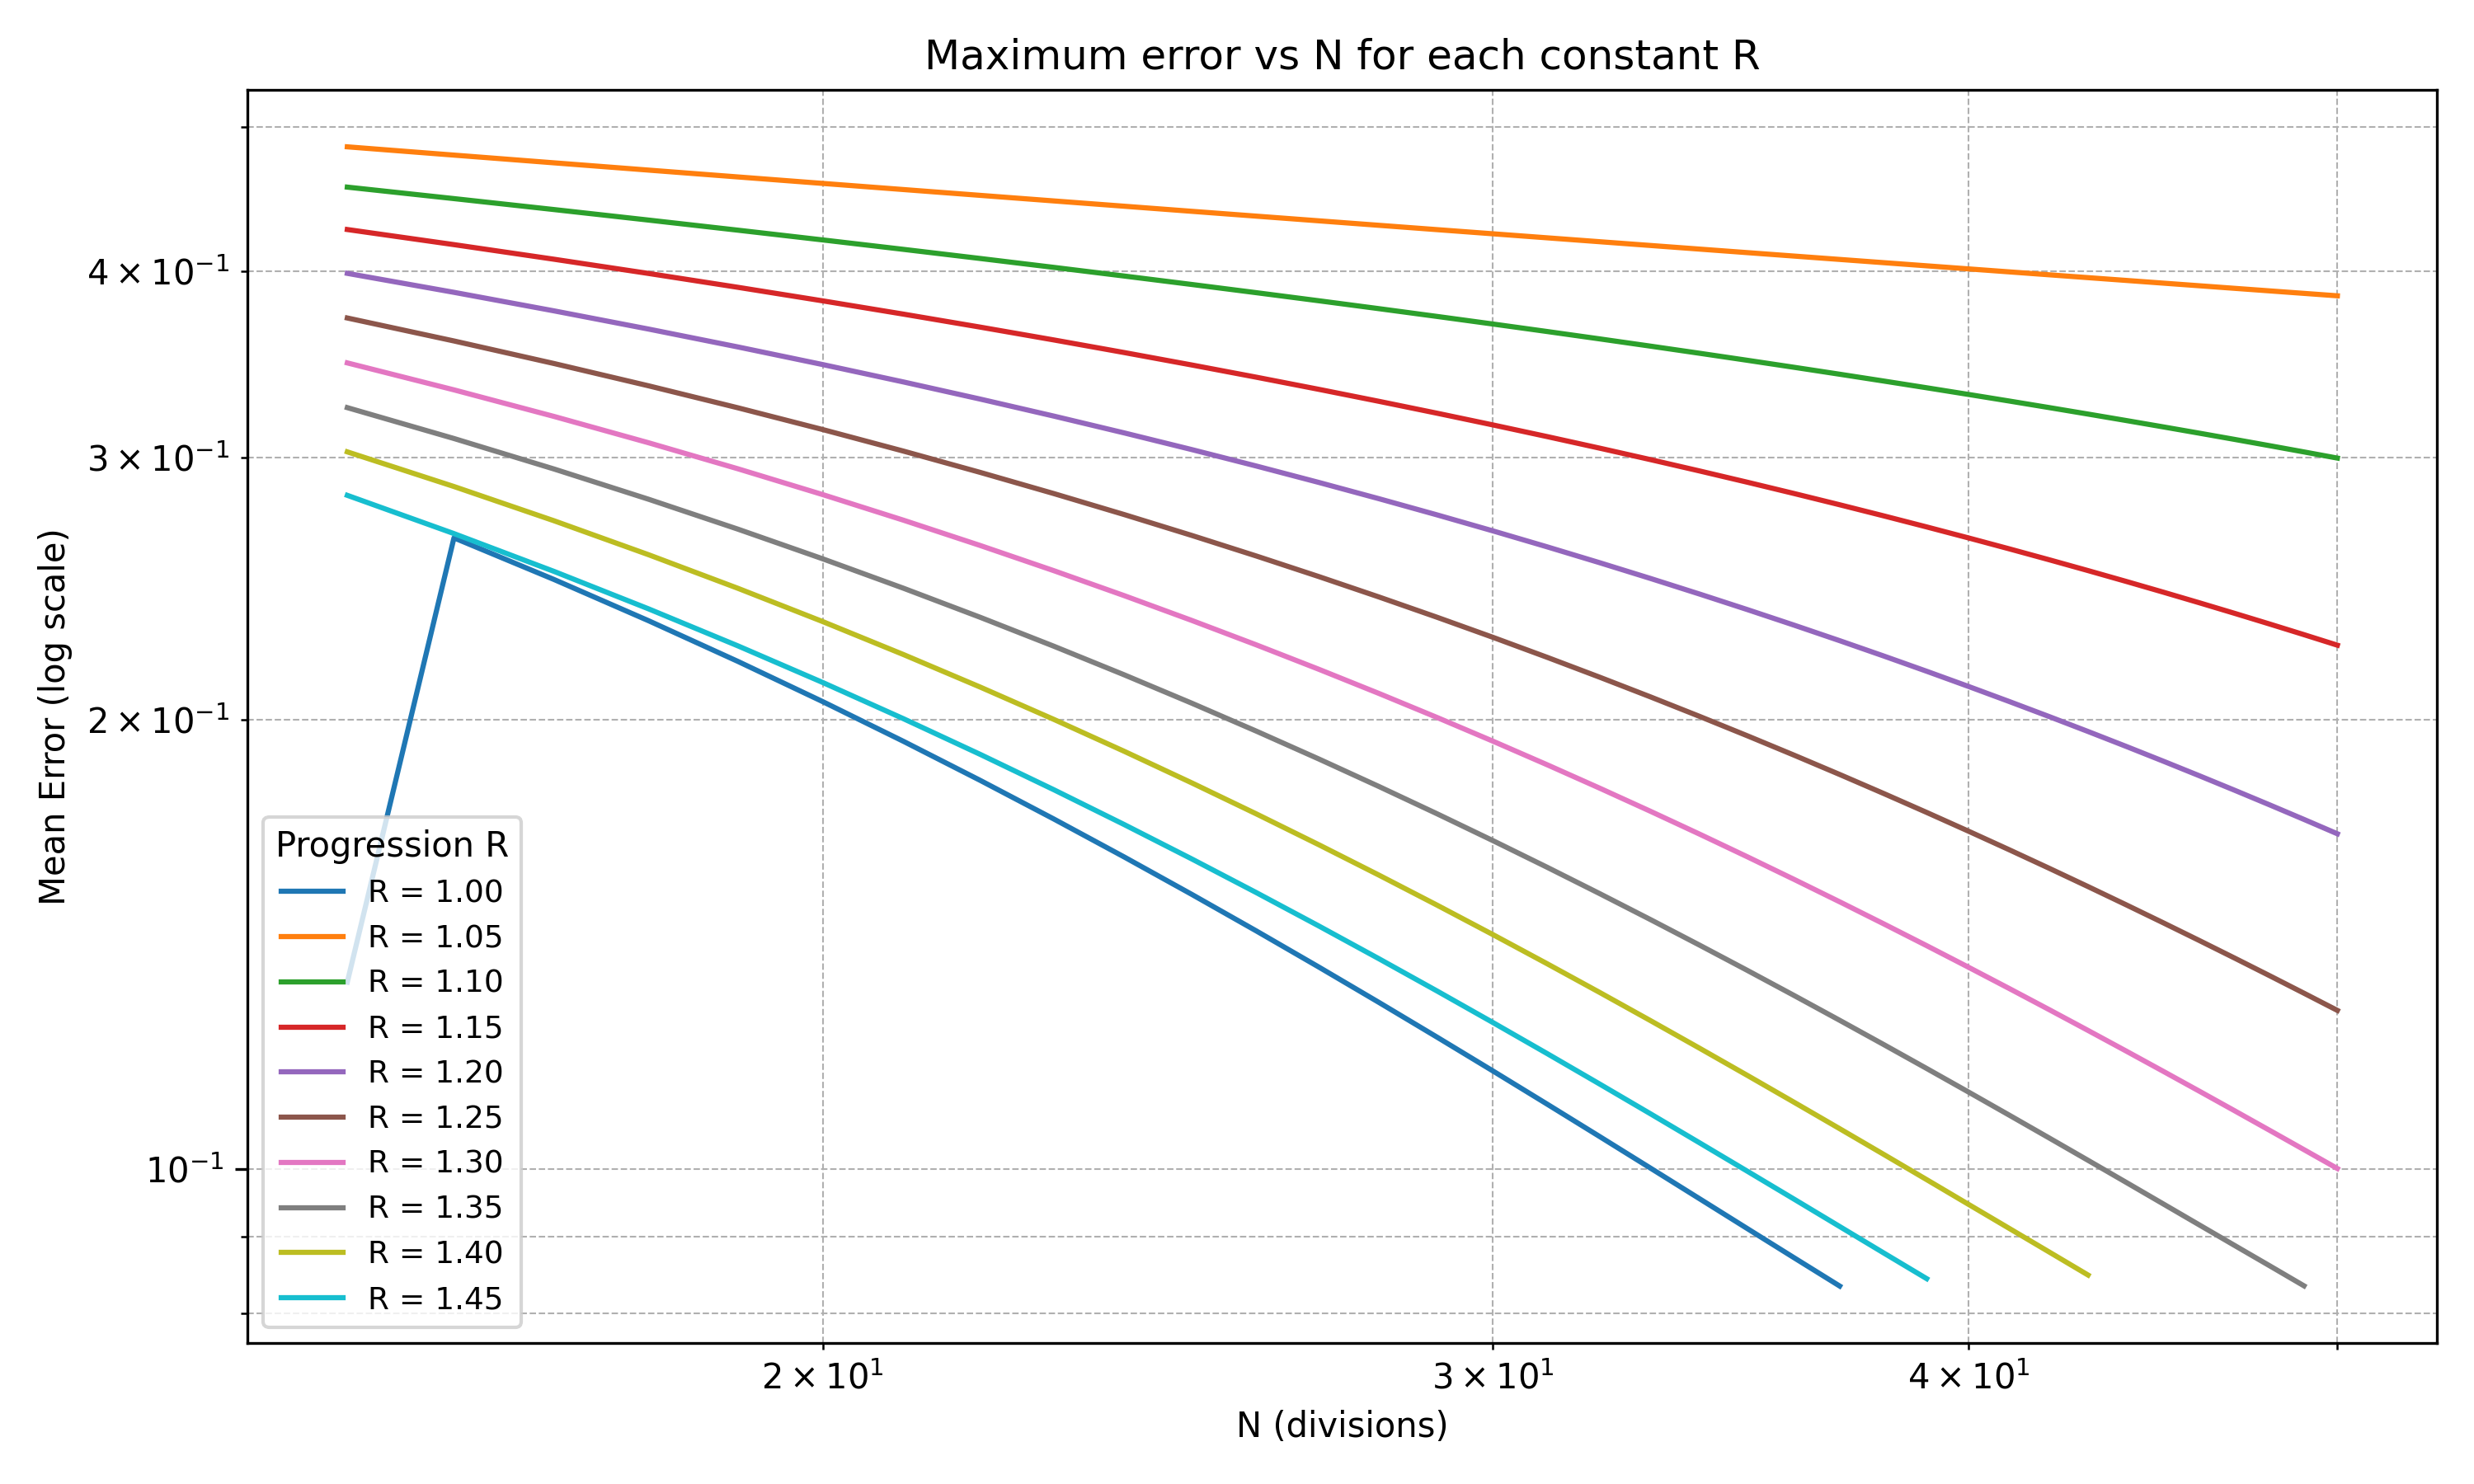
\includegraphics[width=0.6\textwidth]{GRAFICOS/LST/errores_por_R.png}
\caption{Relative error \(\|u - u_h\|_{H^1(\Omega)}\) with varying progression parameter $r$ and $N$ divisions of the mesh for LST elements.}
\label{fig:lst_error_vs_h_loglog} 
\end{figure}

As Figure \ref{fig:lst_comparison} shows, the discrete solution and the analytic solution are smoother and more congruent with each other, this is due to the increase in the ammount of nodes in the LST elements, which allows for a better approximation of the solution. The relative error in Figure \ref{fig:lst_error_vs_h} is also close to 0, but has a smaller singularity response, because of the graeter number of nodes, giving a more uniform approximation of the derivatives of the function. Comparing the error convergence in Figure \ref{fig:lst_error_vs_h_loglog}, we can see that the error decreases faster than the CST elements, due to the quadratic nature of the element.

\newpage
\subsection{Convergence Analysis}

The meshes are generated by subdividing the unit square \(\Omega=(0,1)\times(0,1)\) into \((N-1)\times (N-1)\) triangles whose side lengths along the \(x\) and \(y\) direction follow a geometric progression of ratio \(r\in\{1.00,1.05,1.10\}\).  Concretely, with total length \(L=1\), the first (smallest) element size is
\[
h_{\min} \;=\; S_1 
= \frac{L\,(1 - r)}{1 - r^N},
\]
and the last (largest) element size is
\[
h_{\max} \;=\; S_N
= S_1\,r^{\,N-1}
= \frac{L\,(1 - r)\,r^{\,N-1}}{1 - r^N}.
\]
For \(r=1\) this reduces to the uniform size \(h=1/N\).  For \(r>1\), as \(N\) increases,
\[
h_{\min}\sim\frac{r-1}{r^N}, 
\qquad
h_{\max}\to\frac{r-1}{r},
\]
so the finest element shrinks exponentially with \(N\), while the largest element tends to a constant.

The graded meshes concentrate resolution near one corner by choosing element sizes that decrease geometrically from \(h_{\max}\) at the far boundary down to \(h_{\min}\) so that \(h_{\min}\sim r^{-N}\) decays exponentially in \(N\), while \(h_{\max}\) remains bounded. On such a mesh, the local interpolation error on each triangle scales like \(h_i^p\) (with \(p=1\) for CST), so the error in the smallest elements vanishes faster than any fixed algebraic rate, producing a transient “exponentially convergence” regime visible as a quadratic line segment.  However, once \(h_{\min}^p\) falls below machine precision, the global maximum error is no longer controlled by the finest elements but by those of size \(h_{\max}\), whose error remains \(O(h_{\max}^p)\approx O\bigl((r-1)/r\bigr)^p\), independent of \(N\).  At that point the convergence curve rises and flattens, reflecting the fact that further refinements at the fine end no longer reduces the norm of the error. Thus, geometric grading delivers two distinct regimes; an initial exponential decay phase where \(E\approx C_1\,r^{-pN}\), followed by an increase and latency phase determined by the coarsest element's fixed size. This behavior underscores the trade off inherent in graded meshes: they can dramatically accelerate error reduction in targeted regions, but ultimately yield a global error floor set by the largest remaining element. 


